\chapter{Espectroscopia no infravermelho}

\section{ESPECTRO ELETROMAGNÉTICO}

Discutimos em capítulos anteriores as estruturas de muitos (na verdade, a maior parte) dos tipos conhecidos de compostos orgânicos. No Capítulo 5 evidenciamos a utilidade dos espectros de RMN no estudo dessas estruturas. Um outro grupo de importantes métodos físicos para o estudo de estruturas utiliza o espectro eletromagnético e um desses métodos, aliás dos mais úteis, será discutido em detalhes neste capítulo.

Se uma molécula absorve energia proveniente de radiação eletromagnética pode sofrer vários tipos de \textit{excitação}. A excitação pode causar vários tipos de efeitos: excitação eletrônica, excitação rotacional, mudança de spin nuclear, deformação de ligação, etc. Se a energia disponível se aproxima do potencial de ionização, um elétron pode escapar e ocorre a ionização. Como cada tipo de excitação requer uma quantidade específica energia, a absorção ocorrerá em regiões diferentes do espectro eletromagnético (Tabela \ref{tabela_9_1}).

\begin{table}[H]
\centering
\caption{Espectro electromagnético.}
\label{tabela_9_1}
    \begin{tabular*}{0.9\textwidth}{CCCC}
        \toprule
        Região & Comprimento de onda$^a$ & Energia de excitação ($kcal \cdot mol^{-1}$) & Tipo de excitação \\
        \midrule
        Radiação gama, Raios X, Raios cósmicos & < 100 nm & > 286 &  \\
        \underline{Ultravioleta} &  &  &  \\
        Vácuo & 100-200 nm & 286-143 & Eletrônica \\
        Quartzo & 20-350 nm & 143-82 & Eletrônica \\
        Visível & 350-800 nm & 82-36 & Eletrônica \\
        \underline{Infravermelho$^b$} &  &  & \\
        Infravermelho próximo & 0,8-2,0 $\mu$m & 36-14,3 & Sobretons de deformações de ligação \\
        Infravermelho & 2-16 $\mu$m & 14,3-1,8 & Deformações de ligação \\
        Infravermelho distante & 16-300 $\mu$m & 1,8-0,1 & Deformações de ligação \\
        Microondas & 1 cm & $10^{-4}$ & Rotacional \\
        Radiofrequência & metros & $10^{-6}$ & Transições de spin eletrônico e nuclear \\
        \bottomrule
        \multicolumn{4}{l}{$^a$Veja o Tabela \ref{tabela_9_2} para uma explicação das unidades.} \\
        \multicolumn{4}{p{0.88\textwidth}}{$^b$O espectro Raman pode ser determinado pela exposição da substância a um feixe intenso de radiação de alta energia (usualmente ultravioleta) e medição da luz espalhada pela substância, que é de comprimento de onda diferente do da radiação incidente. Pode-se obter a partir deste espectro o mesmo tipo de informações obtidas do espectro no infravermelho.}
    \end{tabular*}
\end{table}

Quando uma molécula absorve radiação eletromagnética e é excitada de um estado de menor energia a um estado de maior energia, a frequência de absorção é dada pela relação:

\begin{equation}
    E = hv
\end{equation}

\noindent onde $E$ é a energia absorvida, $v$ é frequência radiação eletromagnética e $h$ é a constante de Planck, $6624 \times 10^{-27}\enspace erg \cdot s$. Como a frequência, $v$, e o comprimento de onda, $\lambda$, da radiação absorvida são relacionados, a energia pode ser também expressa em termos de comprimento de onda:

\begin{equation}
    v = \dfrac{c}{\lambda}
\end{equation}
\begin{equation}
    E = hv = \dfrac{hc}{\lambda}
\end{equation}

\noindent onde $\lambda$ é o comprimento de onda, e $c$ é a velocidade de luz, $2998 \times 10^{10}$ centímetros por segundo ($cm \cdot s^{-1}$). O número de ondas, $n$, é definido como o inverso do comprimento de onda em centímetros e é normalmente usado em substituição ao comprimento de onda porque os valores numéricos são de magnitude conveniente:

\begin{equation}
    n = \dfrac{1}{\lambda}
\end{equation}

\noindent onde $n$ é em cm$^{-1}$.

As regiões de ultravioleta e infravermelho podem ser subdivididas em sub-regiões, como é mostrado na Tabela \ref{tabela_9_1}. A relação $E = \dfrac{hc}{\lambda}$ mostra que a energia de excitação é inversamente proporcional ao comprimento de onda. Assim, quando o comprimento de onde aumenta na Tabela \ref{tabela_9_1} a energia decresce. As energias maiores (menores comprimentos de onda) do que as encontradas na região do ultravioleta, a energia poderá ser suficiente para ionizar a molécula ou mesmo causar transformações nucleares.

Os termos \textit{espectrometria} e \textit{espectroscopia} são sinônimos. Um \textit{espectrofotômetro} é o instrumento usado para medir os espectros no ultravioleta, visível e infravermelho. O instrumento usado para medir os espectros de ressonância magnética nuclear ou de massas é usualmente chamado de \textit{espectrômetro}. Outros símbolos e termos correntemente utilizados estão definidos no Tabela \ref{tabela_9_2}.

\begin{table}[H]
\centering
\caption{Abreviaturas e definições.}
\label{tabela_9_2}
    \begin{tabular*}{0.8\textwidth}{cc}
        \toprule
        Abreviaturas & Definição \\
        \midrule
        UV & Ultravioleta \\
        IV & Infravermelho \\
        \AA & A unidade Angstrom, igual a $10^{-8}$ centímetros \\
        $\mu$m$^a$ & A unidade micrômetro, igual a $10^{-6}$ metros\\
        nm & A unidade nanômetro, igual a $10^{-9}$ metros \\
        cm$^{-1}$ & A unidade centímetro inverso, igual ao inverso de um centímetro \\
        \bottomrule
        \multicolumn{2}{p{0.78\textwidth}}{$^a$As unidades mícron ($\mu$) e milimícron (m$\mu$) eram usadas na antiga literatura e estão atualmente sendo substituídas pelos seus equivalentes micrômetro e nanômetro, respectivamente.}
    \end{tabular*}
\end{table}

\noindent É importante enfatizar que para cada tipo de excitação uma \textit{quantidade definida de energia é necessária}. Estes fenômenos são quantizados. Assim uma radiação de frequência determinada e característica é absorvida para uma determinada transição. A interpretação de um espectro de absorção é baseada na associação da absorção de energia à presença de determinados grupos estruturais na molécula. Dados obtidos dos espectros de absorção, embora úteis, nem sempre são suficientes para levar à estrutura completa e correta da molécula sob exame. Tais dados são mais eficazes quando usados juntamente com dados químicos.

\section{ESPECTROS NO INFRAVERMELHO}

A divisão da região do espectro eletromagnético correspondente ao infravermelho em três sub-regiões, infravermelho próximo, infravermelho e infravermelho distante, é baseada arbitrariamente no desenho e custo do instrumento. Nós discutiremos a região de comprimento de onda 2,5 a 16 $\mu$m (em termos de número de ondas, 4000 a 625 cm$^{-1}$) porque é região usada habitualmente pelo químico orgânico no trabalho de identificação de estruturas.

A Figura \ref{figura_9_1} apresenta o diagrama esquemático de um espectrofotômetro. É possível obter-se a intensidade de radiação que penetra o tubo da amostra a partir da intensidade do feixe de referência, que é a mesma do feixe incidente. A diferença entre a intensidade do feixe referência e a do feixe transmitido mede a quantidade de radiação absorvida. A frequência da radiação sob exame é variada automaticamente pelo \textit{monocromador}. No \textit{fotômetro} são comparadas às intensidades relativas dos feixes transmitido e de referência e a percentagem obtida é lançada em gráfico como função do número de ondas.

\begin{figure}[H]
    \centering
    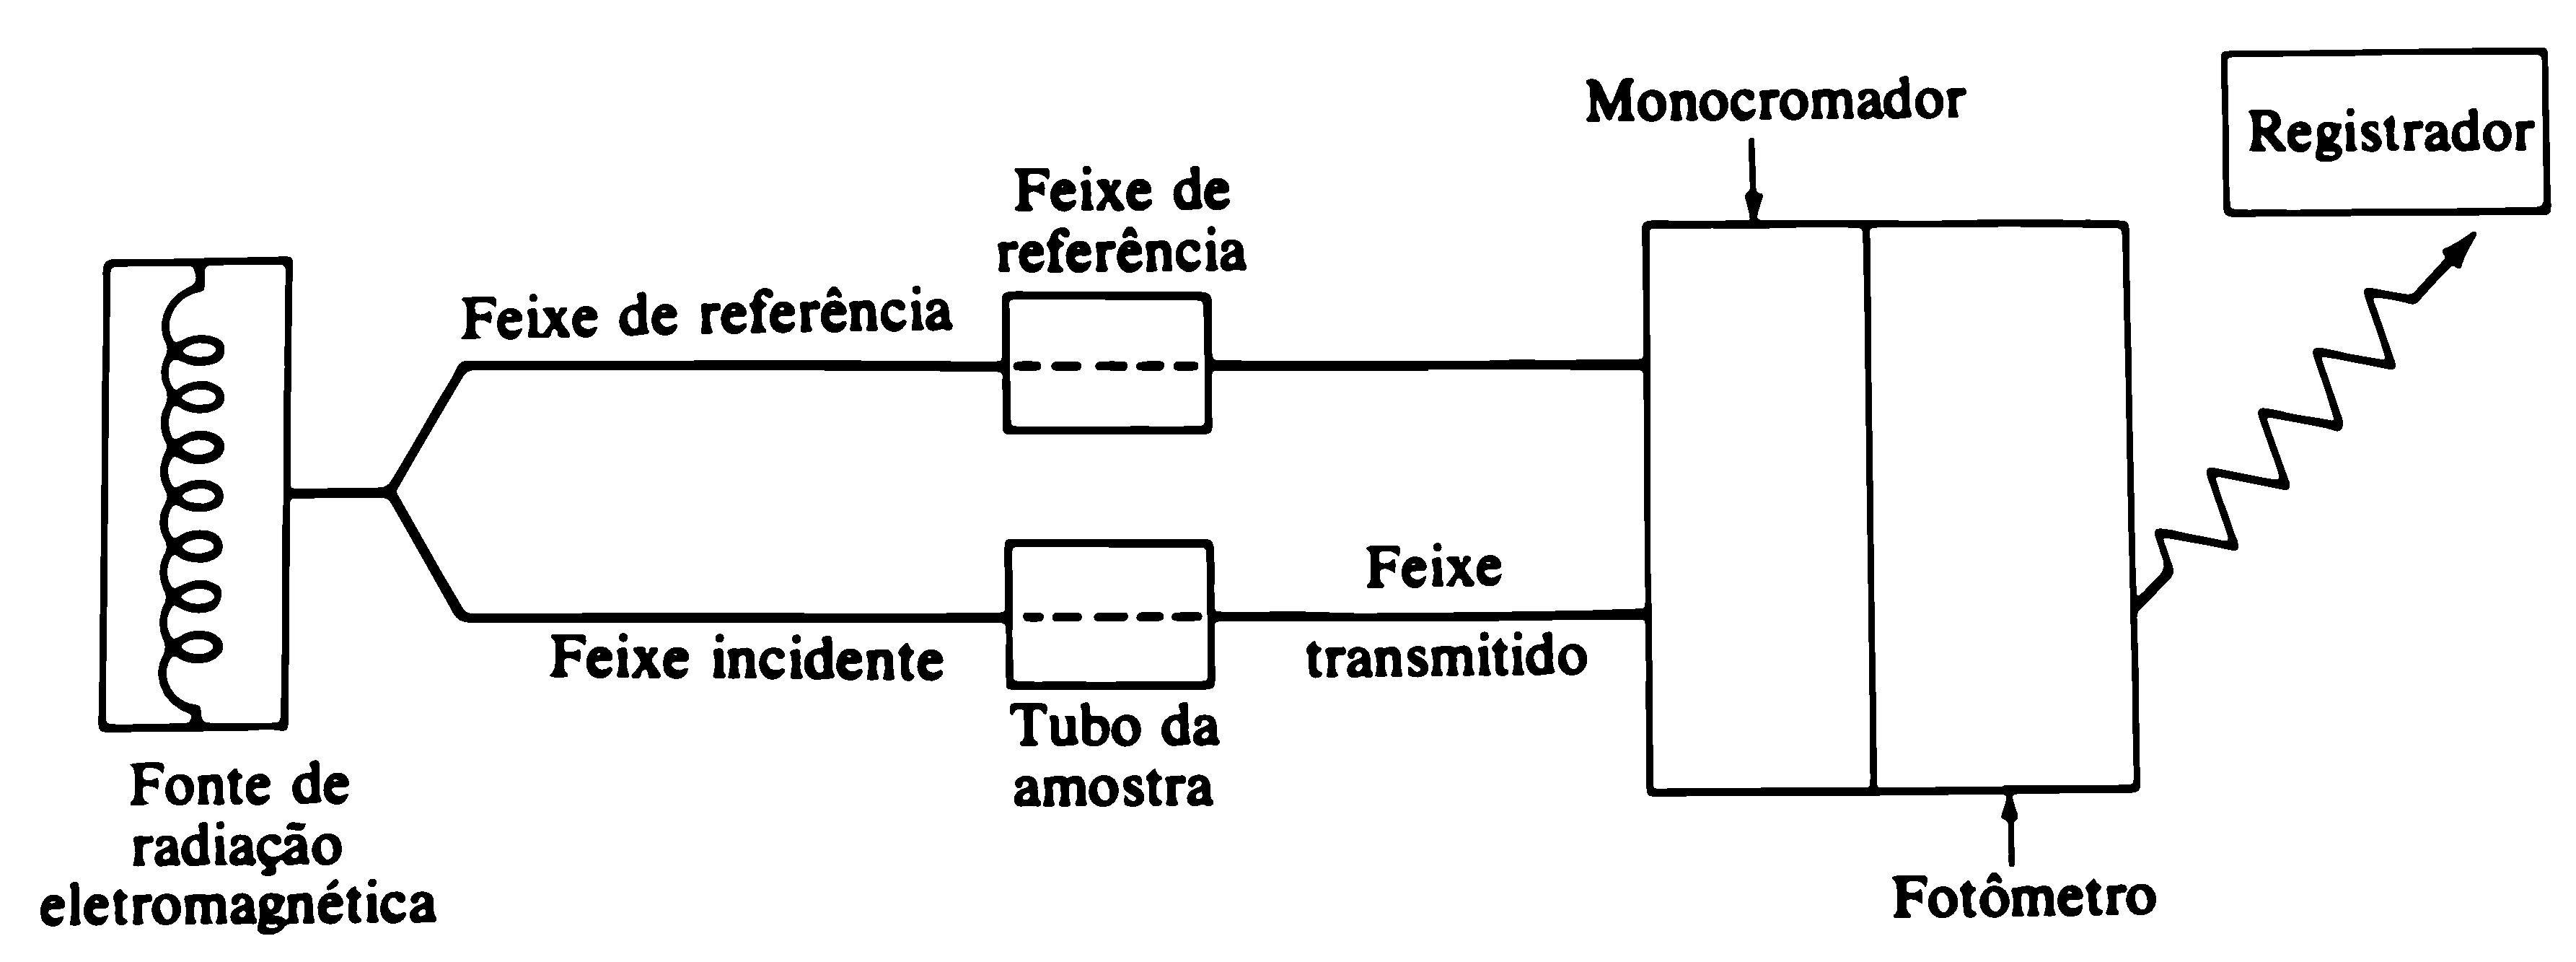
\includegraphics[width=0.9\textwidth,angle=0]{content/images/Figura_9_1.pdf}
    \caption{Diagrama esquemático de um espectrofotômetro simples.}
    \label{figura_9_1}
\end{figure}

A Figura \ref{figura_9_2} mostra o espectro do $n$-hexano no infravermelho. Note que é habitual apresentar o espectro em função da luz transmitida (de 0 a 100\%) e não em função da luz absorvida. Assim, os espectros no infravermelho mostram absorção \textit{máxima} nos \textit{mínimos} do gráfico, ao contrário dos espectros de RMN onde é habitual usar-se absorção.

\begin{figure}[H]
    \centering
    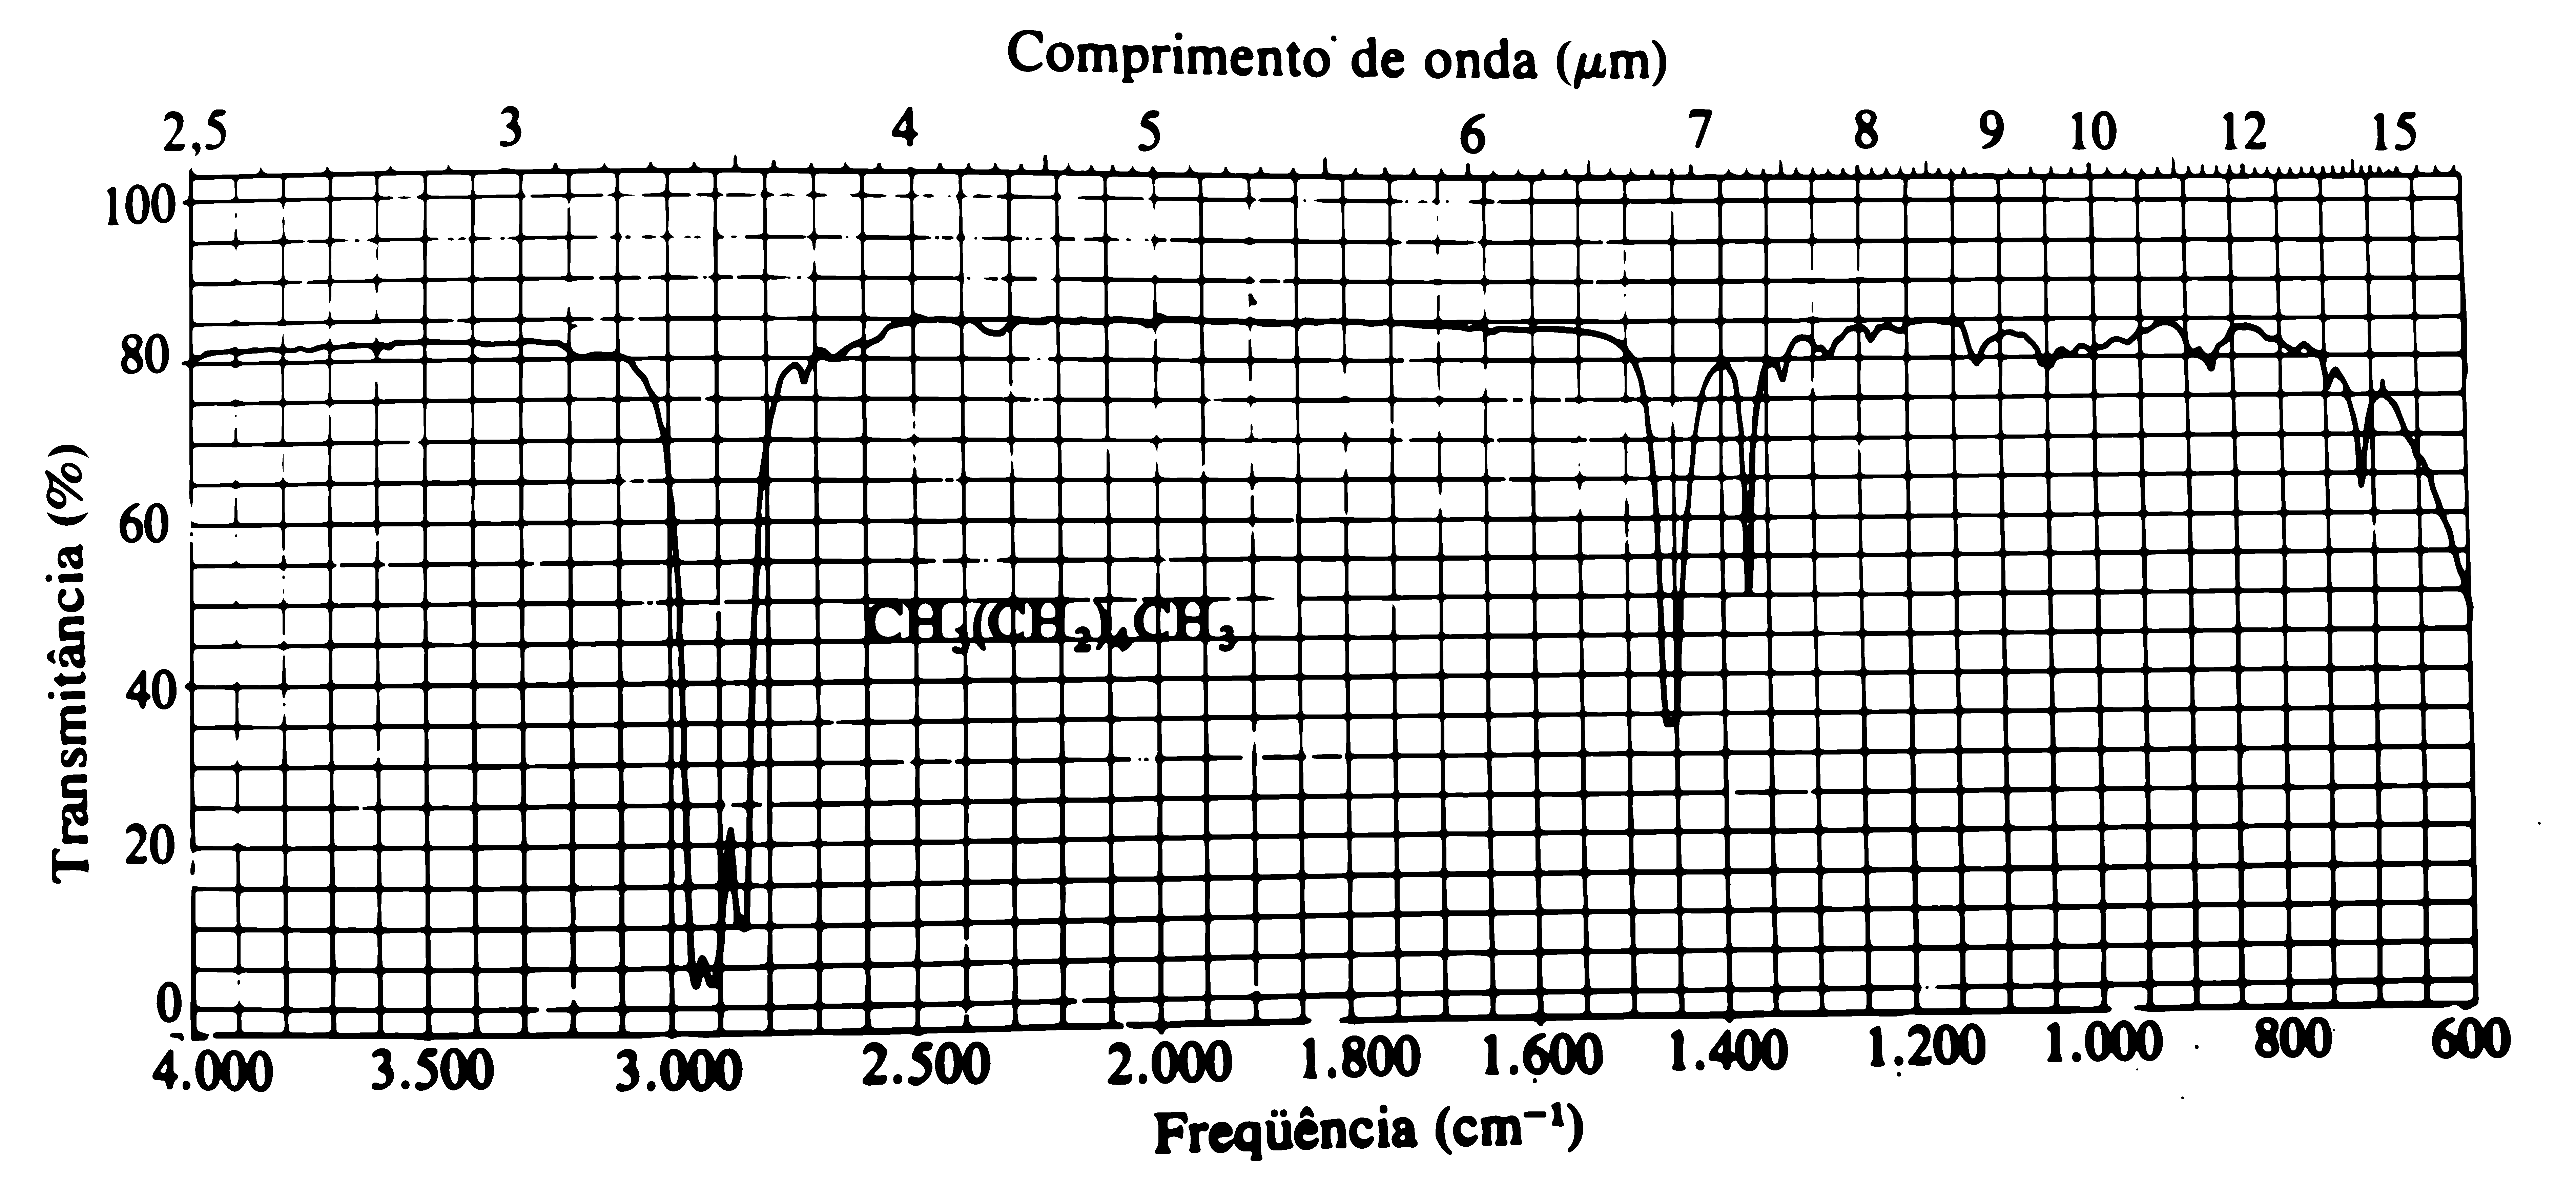
\includegraphics[width=0.9\textwidth,angle=0]{content/images/Figura_9_2.pdf}
    \caption{Espectro do $n$-hexano no infravermelho (filme líquido).}
    \label{figura_9_2}
\end{figure}

Em muitos partes do gráfico a transmitância é próxima de 100\%, significando que a substância é transparente à radiação daquelas frequências. Note as fortes bandas de absorção a 2900 a 1450 cm$^{-1}$, que resultam dos movimentos de deformação axial e angular da ligação \ch{C-H}, respectivamente. As bandas de absorção não são linhas finas porque os níveis de energia vibracional têm a eles associados um certo número de níveis rotacionais e as transições entre estes níveis causam o alargamento das bandas.

O espectro de substâncias no infravermelho pode ser obtido nos estados \textit{líquido} (líquidos homogêneos não contendo solventes), no gasoso ou sólido ou, ainda, em solução. No caso de espectros de soluções um tubo contendo \textit{apenas} o \textit{solvente} pode ser colocado no feixe de referencia (Figura \ref{figura_9_1}). A absorção do solvente no feixe incidente é compensada pela absorção no feixe referência e obtém-se assim o registro apenas do soluto.

A energia absorvida na excitação de uma molécula a um estado de energia mais alto é liberada quando a molécula retorna a um estado de energia mais baixo. Na região do infravermelho a energia é liberada sob a forma de calor, o que causa um aumento temperatura da amostra.

Diferentes tipos de átomos têm diferentes massas. Diferentes tipos de ligações têm forças de ligação diferentes, as quais aproximadamente independentes dos átomos que não participam diretamente da ligação sob exame (exceto no caso de sistemas conjugados e outros casos especiais). Logo, combinações diferentes de masses atômicas e energias de ligação dão origem a sistemas que vibram a frequências diferentes quando a molécula absorve energia eletromagnético. Por exemplo, o sistema de ligações, \ch{O-C-O} do dióxido de carbono absorve energia de número de ondas 667 cm$^{-1}$ quando há deformação angular, enquanto no sistema \ch{H-O-H} o mesmo acontece a 1595 cm$^{-1}$.

\begin{figure}[H]
    \centering
    \chemnameinit{}
    \chemname[0.8ex]{\chemname[2ex]{\chemfig[][scale=0.7]{\chemabove{O}{\footnotesize\uparrow}=\chembelow{C}{\footnotesize\downarrow}=\chemabove{O}{\footnotesize\uparrow}}}{\footnotesize{Deformação angular de \ch{O-C-O}}}}{\footnotesize{$n$ = 667 cm$^{-1}$}}
    \chemnameinit{}
    \qquad\qquad\qquad\qquad
    \chemname[0.8ex]{\chemname{\chemfig[][scale=0.7]{\chemabove{H}{\footnotesize\nwarrow}(-[1]\chembelow{O}{\footnotesize\downarrow}(-[7]\chemabove{H}{\footnotesize\nearrow}))}}{\footnotesize{Deformação angular de \ch{H-O-H}}}}{\footnotesize{$n$ = 1595 cm$^{-1}$}}
    \chemnameinit{}
\end{figure}

Os diferentes movimentos vibracionais dos átomos de uma molécula podem levar também à absorção em diferentes números de onda. Considere, por exemplo, a molécula da água. Os movimentos dos dois hidrogênios não são independentes, havendo um acoplamento entre eles, como acontece com dois pêndulos com suas origens na mesma barra. Este acoplamento leva a um movimento simétrico, no qual os dois hidrogênios se afastam e se aproximam ao mesmo tempo, e a um movimento assimétrico, no qual um dois hidrogênios se aproxima do oxigênio enquanto o outro se afasta. Uma ligação \ch{O-H} isolada, isto é, sem os efeitos do acoplamento, teria uma vibração de deformação axial absorvendo a 3700 cm$^{-1}$ (equidistante das vibrações simétrica e assimétrica). A mudança em qualquer um desses movimentos requer absorção de diferentes quantidades de energia, o que leva à absorção em frequências características do espectro no infravermelho. Assim, a molécula \ch{H2O} tem um total de três absorções características a frequências diferentes:

\begin{figure}[H]
    \centering
    \chemnameinit{}
    \chemname[0.8ex]{\chemname[2.5ex]{\chemfig[][scale=0.7]{\chembelow{H}{\footnotesize{\swarrow}}(-[1]O(-[7]\chembelow{H}{\searrow}))}}{\footnotesize{Deformação axial simétrica}}}{\footnotesize{$n$ = 3655 cm$^{-1}$}}
    \chemnameinit{}
    \qquad\qquad\qquad\qquad
    \chemname[0.8ex]{\chemname[2.5ex]{\chemfig[][scale=0.7]{\chembelow{H}{\footnotesize{\swarrow}}(-[1]O(-[7]\chembelow{H}{\nwarrow}))}}{\footnotesize{Deformação axial assimétrica}}}{\footnotesize{$n$ = 3756 cm$^{-1}$}}
    \chemnameinit{}
    \qquad\qquad\qquad\qquad
    \chemname[0.8ex]{\chemname[2.5ex]{\chemfig[][scale=0.7]{\chemabove{H}{\footnotesize{\nwarrow}}(-[1]O(-[7]\chemabove{H}{\nearrow}))}}{\footnotesize{Deformação angular}}}{\footnotesize{$n$ = 1595 cm$^{-1}$}}
    \chemnameinit{}
\end{figure}

\noindent\textbf{Espectro de hidrocarbonetos no infravermelho}

O acoplamento de frequências vibracionais ocorre mais efetivamente quando as frequências são próximas. Nas moléculas orgânicas há usualmente muitas ligações \ch{C-C} e \ch{C-H} e as frequências de vibração dos átomos geralmente se acoplam dando um espectro muito complicado. Entretanto, certas características são identificáveis nos espectros dos hidrocarbonetos. No espectro do $n$-hexano (Figura \ref{figura_9_2}), as bandas de absorção mais fortes são observadas a 2900 e 1450 cm$^{-1}$, originando-se nas deformações axial e angular, respectivamente. Todos as moléculas que contêm grupos alquila mostram essas bandas de absorção que são, portanto, encontradas em quase todos os espectros de compostos orgânicos no infravermelho. A deformação angular simétrica de um a grupamento metila leva à absorção a aproximadamente 1380 cm$^{-1}$. O grupamento metila terminal de grupamentos alquila mostra esta absorção e consequentemente uma banda a 1380 cm$^{-1}$ é encontrada na maioria dos espectros de compostos orgânicos.

A ligação \ch{C+C} é mais forte do que ligação \ch{C=C} e em consequência a deformação axial é mais difícil. A formação axial da ligação \ch{C+C} é responsável, portanto, pela absorção a um número de ondas mais alto do que a deformação axial da ligação \ch{C=C}. Esta última, por outro lado, causa absorção a um número de onda mais alto do que a deformação axial ligação \ch{C-C}. Graças ao acoplamento dos modos de vibração de deformação axial das ligações \ch{C-C} e \ch{C-H}, a região 1.400-800 cm$^{-1}$ do espectro de uma molécula tipica é usualmente muito complicada e as bandas não podem ser individualmente associadas a determinadas ligações. Por outro lado, esta região é característica de uma determinada molécula. Esta parte do espectro é conhecido como a região da impressão digital, por razões óbvias.

\noindent MATÉRIA OPCIONAL
Relações entre as frequências vibracionais e as propriedades de ligação. Em uma aproximação grosseira todas as ligações simples têm forças de ligação ou constantes de força de deformação axial semelhantes e a energia para esta deformação é dada por:

\begin{equation}
    E = \dfrac{1}{2}k(\delta l )^2
\end{equation}

A constante $K$ é chamada a constante de força e mede a resistência de ligação ao movimento de deformação axial. A quantidade $\delta l$ é uma medida da extensão da deformação. Este tipo de relação é o mesmo que descreve classicamente o movimento de duas massas ligadas por molas (lei do Hooke).

Para ligações duplas, \ch{X=Y}, as constantes de força são mais ou menos o dobro das observadas para ligações simples e para ligações triplas, \ch{X+Y}, o triplo. A frequência vibracional da ligação \ch{X-Y} em cm$^{-1}$, quando a massa de Y é muito maior do que a da X, é dada por:

\begin{equation}
    v = \dfrac{1}{2 \pi c}\sqrt{\dfrac{k}{m_x}}
\end{equation}

\noindent onde $k$ é a constante de força para a deformação axial, $m_x$ é massa do átomo X, e $c$ é a velocidade da luz. Para X constante as razões das frequências de vibração de \ch{X-Y}, \ch{X=Y} e \ch{X+Y} são aproximadamente 1, $\sqrt{2}$ e $\sqrt{3}$. Note, também, que quando $m_x$ aumenta a frequência diminui, porque neste caso é proporcional a $\dfrac{1}{\sqrt{m_x}}$. Como a massa do hidrogênio é pequena, as frequências de vibração de deformação axial da ligações \ch{H-Y} são excepcionalmente altas.

Podemos agora construir o diagrama sumariando as regiões de absorção no infravermelho de ligações carbono-carbono e carbono-hidrogênio (Figura 9.3). A absorção de deformação axial de \ch{C-H} ocorre próxima a 2900 cm$^{-1}$ (alquila), 3100 cm$^{-1}$ (vinila) e 3300 cm$^{-1}$ (\ch{H-C+C\bond{normal}}).

\begin{figure}[H]
    \centering
    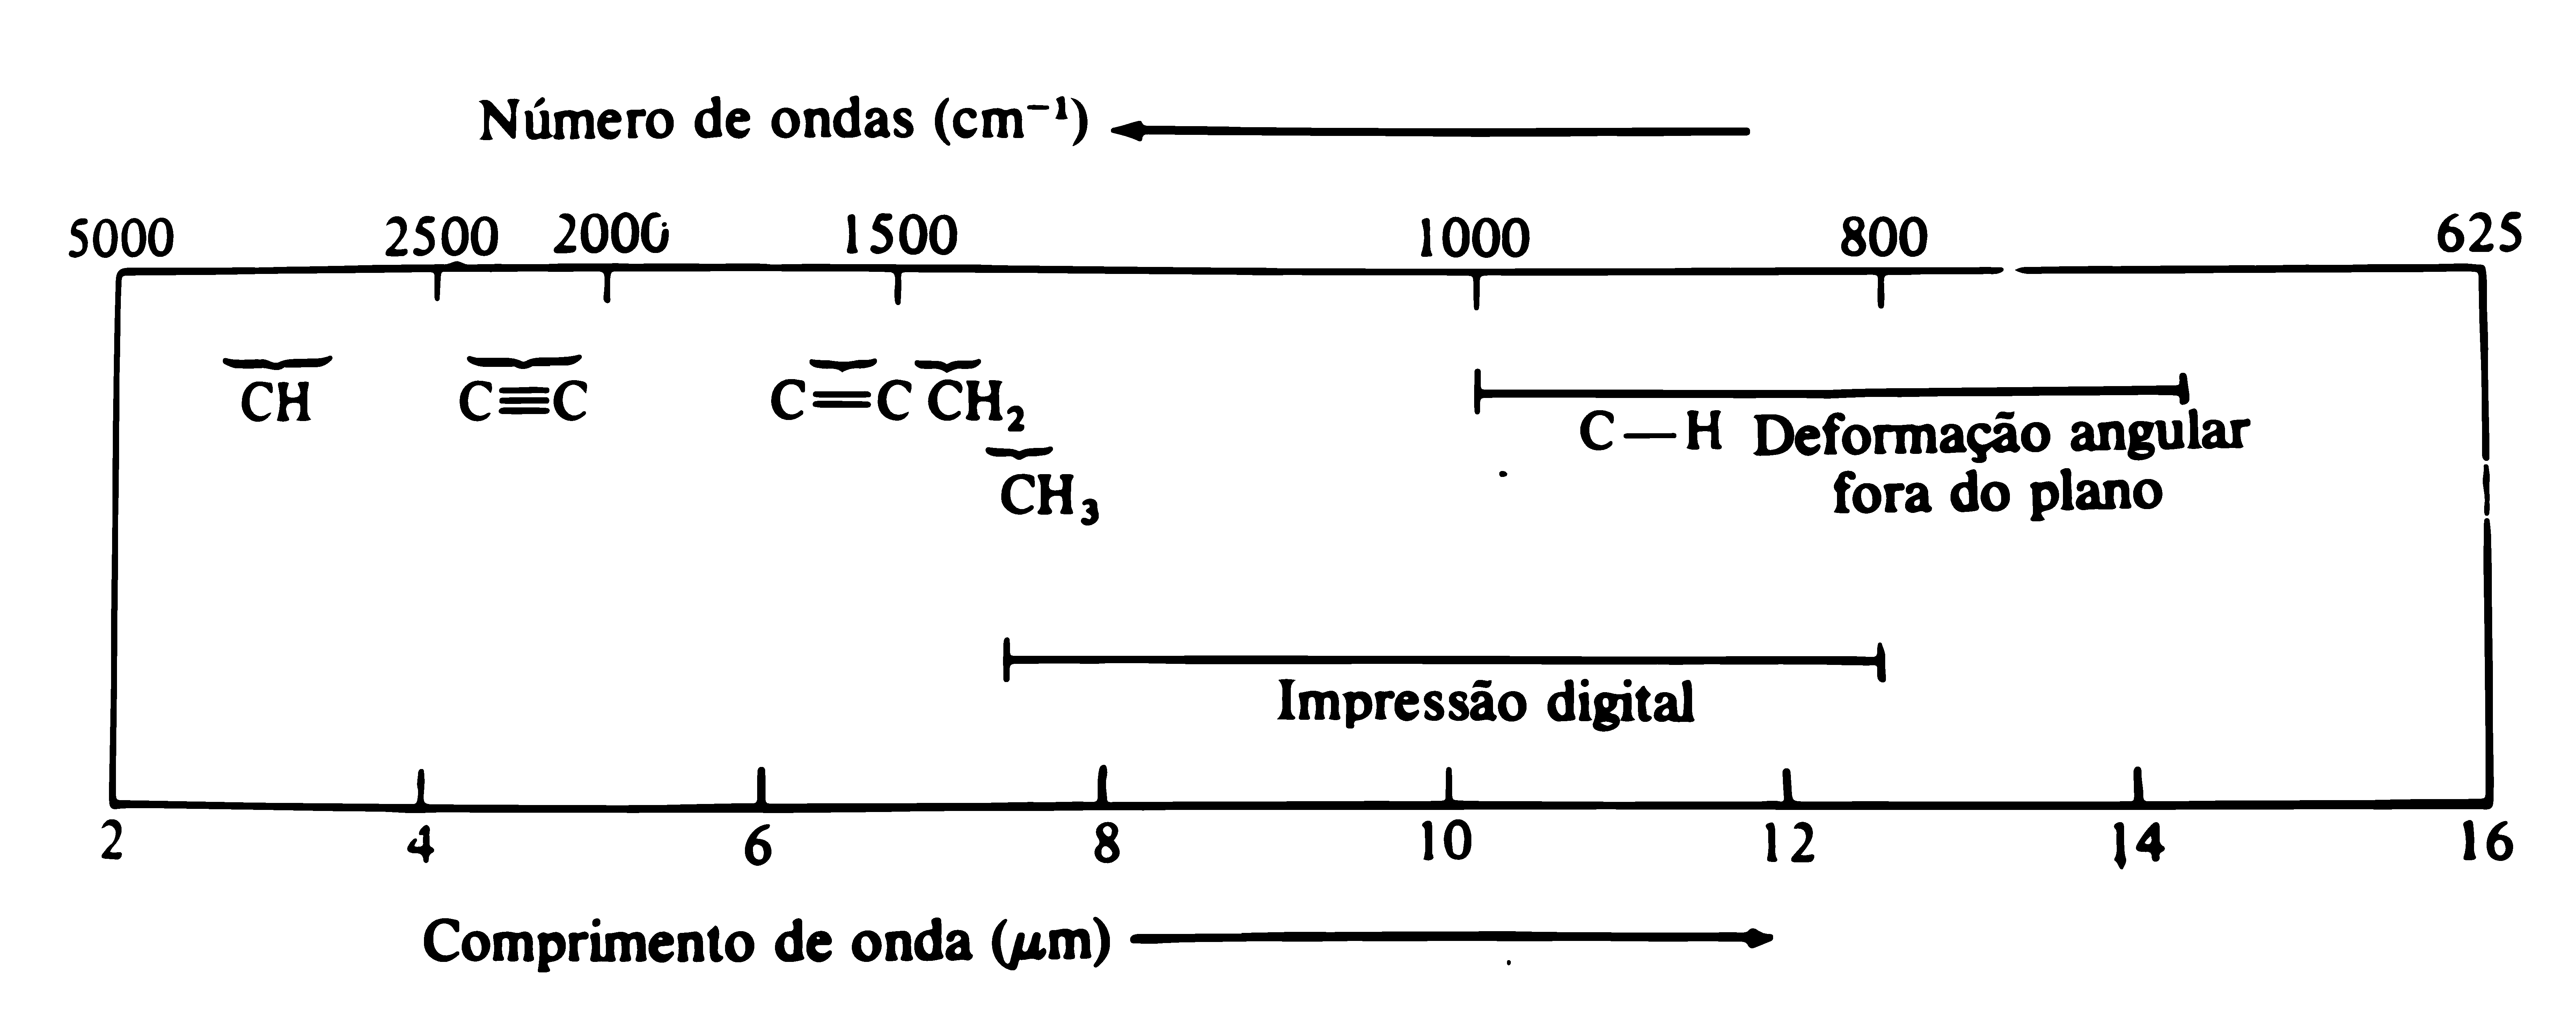
\includegraphics[width=0.9\textwidth,angle=0]{content/images/Figura_9_3.pdf}
    \caption{Regiões de absorção de ligações \ch{C-C} e \ch{C-H} no infravermelho.}
    \label{figura_9.3}
\end{figure}

Ligações triplas absorvem a 2300-2100 cm$^{-1}$ e ligações duplas próximas a 1650 cm$^{-1}$. Hidrogênios vinílicos mostram bandas fortes correspondendo às 'deformações angulares fora do plano' na região 1000-700 cm$^{-1}$. Muitas destas características aparecem no espectro do metileno-ciclo-hexano (Figura \ref{figura_9_4}).

\noindent\textbf{Espectro IV de grupos funcionais}

\noindent Os espectros de infravermelho são regularmente usados pelos químicos orgânicos para facilitar a identificação de grupos funcionais. Comparando os espectros das Figuras \ref{figura_9_4}-\ref{figura_9_7} vemos como a presença e a ausência de absorções específicas podem ser usadas para reconhecer-se a presença ou a ausência de determinado grupo funcional em uma molécula.

O espectro no infravermelho do 1-hexanol (Figura \ref{figura_9_5}) ilustra a absorção de deformação axial característica da hidroxila de um álcool em ligação hidrogênio - a banda larga e forte a 3330 cm$^{-1}$ e mostra também a absorção da ligação \ch{C-O} a 1060 cm$^{-1}$. Em contraste, o espectro do dietil-éter (Figura 9.6) não apresenta a absorção da hidroxila a 3330 cm$^{-1}$ mas tem uma absorção forte a 1125 cm$^{-1}$, característica da deformação axial da ligação \ch{C-O}.

O espectro do butirato de etila no infravermelho (Figura \ref{figura_9_7}) mostra absorção forte na região de 1730 cm$^{-1}$ atribuída à vibração de deformação axial da carbonila. A Figura \ref{figura_9_7} não mostra, por outro lado, a banda característica da deformação axial de \ch{O-H} de álcoois em ligação hidrogênio a 3330 cm$^{-1}$ (Figura \ref{figura_9_5}), mas tem a deformação axial de \ch{C-O} a 1180 cm$^{-1}$ (Figura \ref{figura_9_6}). As Figuras \ref{figura_9_4}-\ref{figura_9_6} não mostram a absorção forte a 1.730 cm$^{-1}$ característica de \ch{C=O} (Figura \ref{figura_9_7}). Podemos concluir que o composto da Figura \ref{figura_9_7} contém um grupo carbonila, o que não acontece com os das Figuras \ref{figura_9_4}-\ref{figura_9_6}, que a Figura \ref{figura_9_4} corresponde a um composto não contém nenhum dos grupos funcionais que aparecem nas Figuras 9.5-9.7, e que todos os compostos das Figuras \ref{figura_9_5}-\ref{figura_9_7} contêm ligações \ch{C-O}. Deste modo, os químicos podem comparar os espectros de compostos conhecidos com espectros de compostos desconhecidos e, frequentemente, identificar os grupos funcionais presentes nos desconhecidos.

\begin{figure}[H]
    \centering
    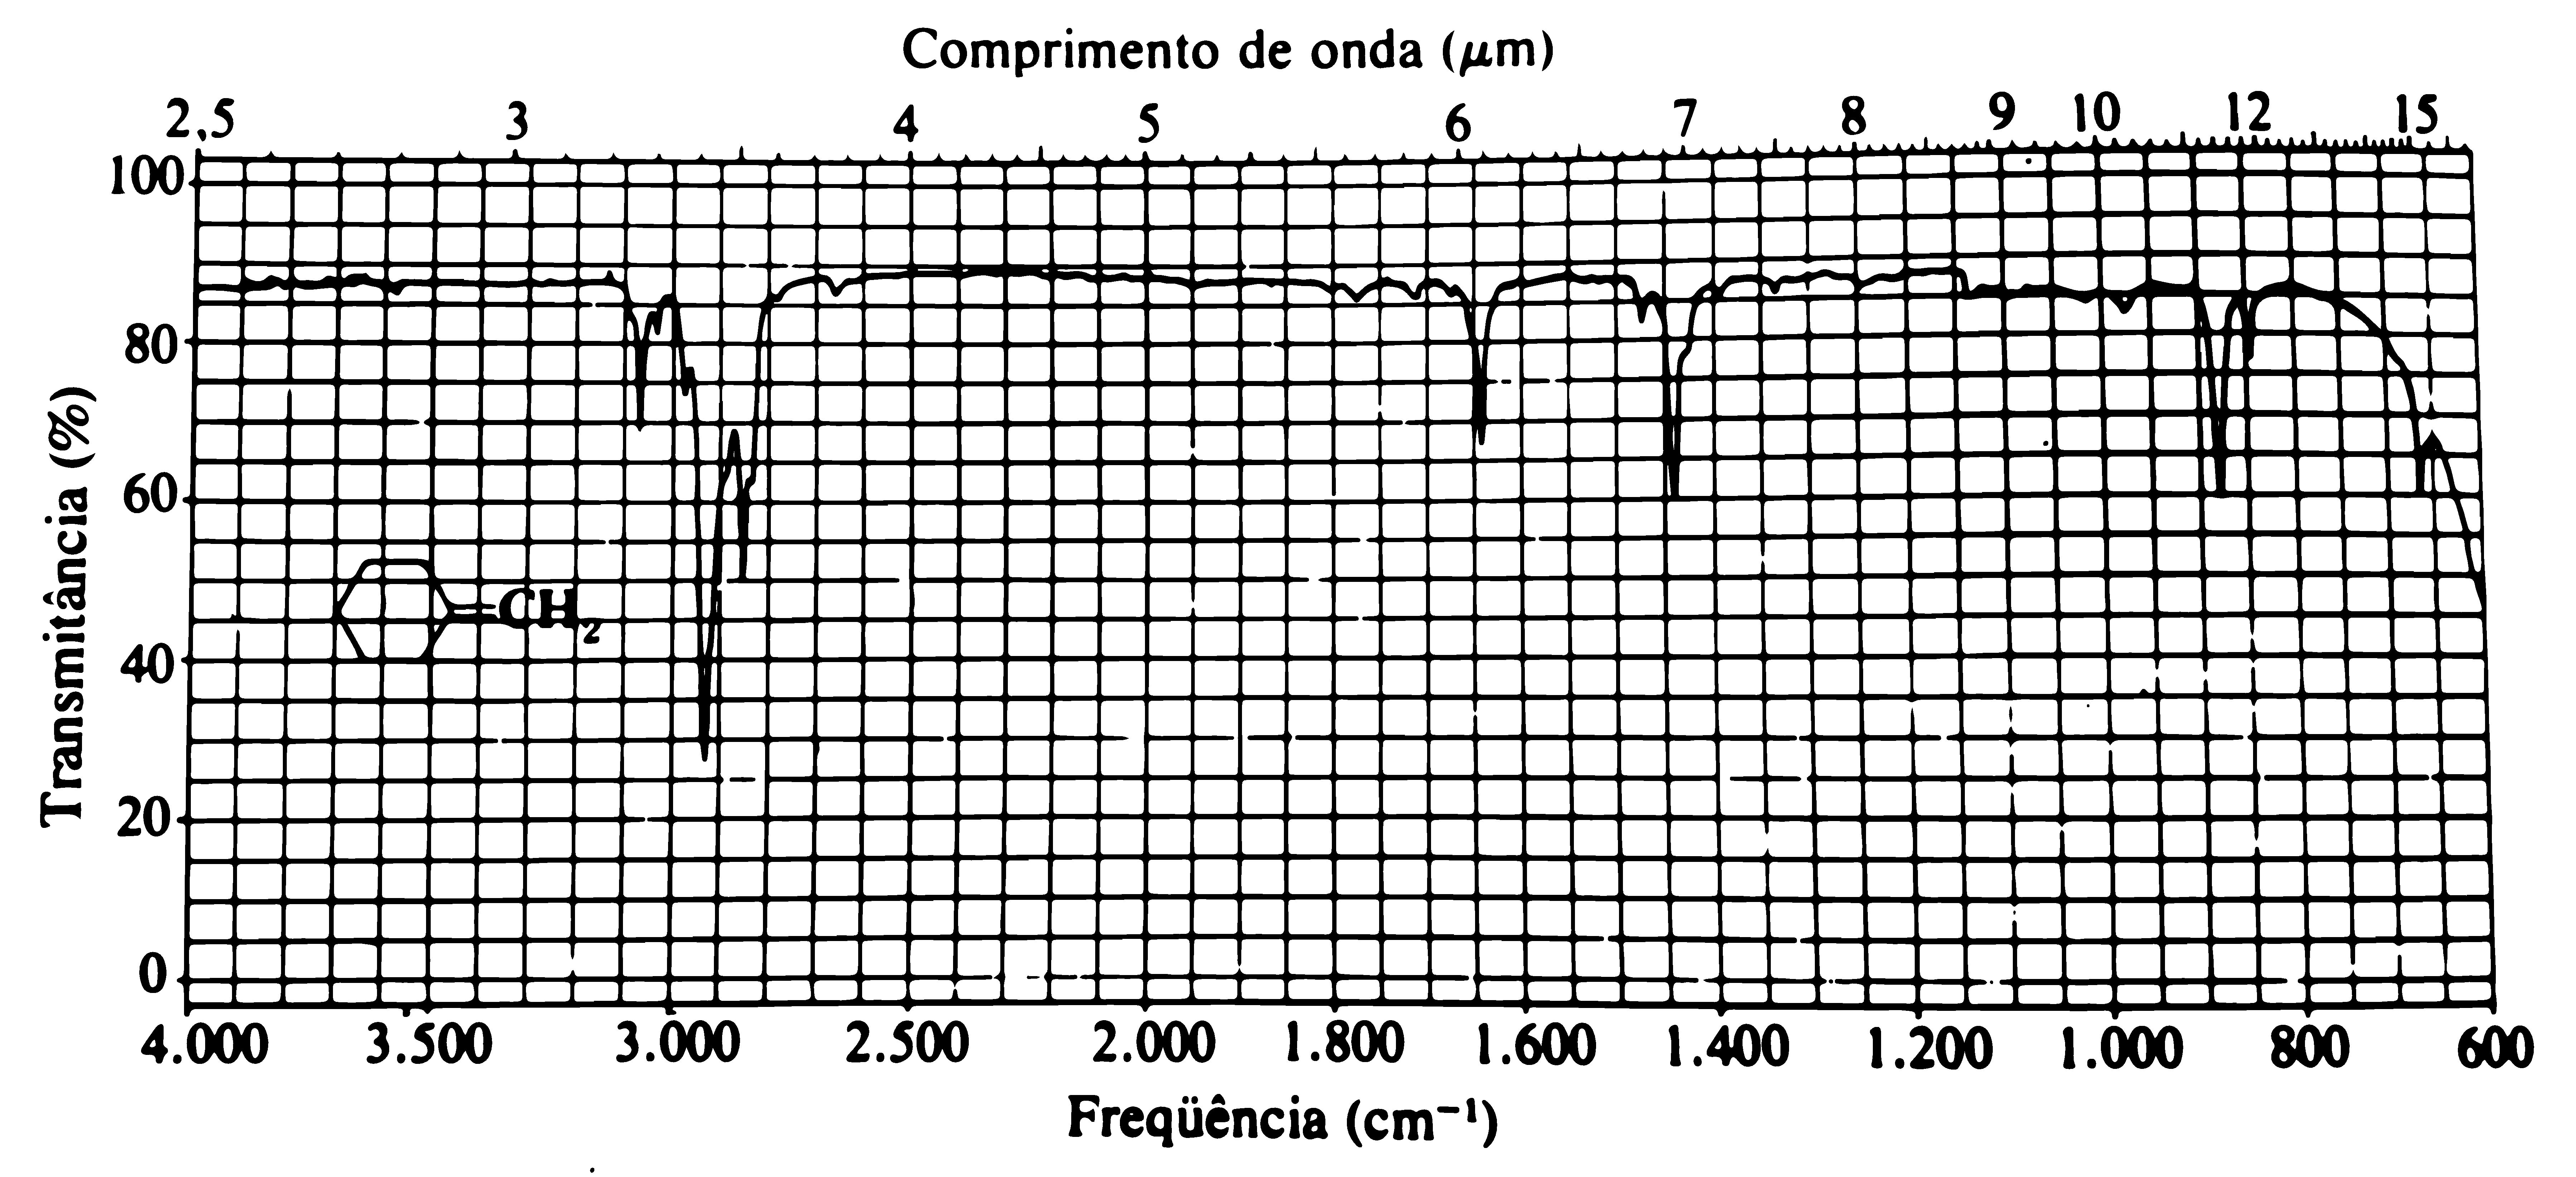
\includegraphics[width=0.85\textwidth,angle=0]{content/images/Figura_9_4.pdf}
    \caption{Espectro do metileno-ciclo-hexano no infravermelho (filme líquido).}
    \label{figura_9_4}
\end{figure}

\begin{figure}[H]
    \centering
    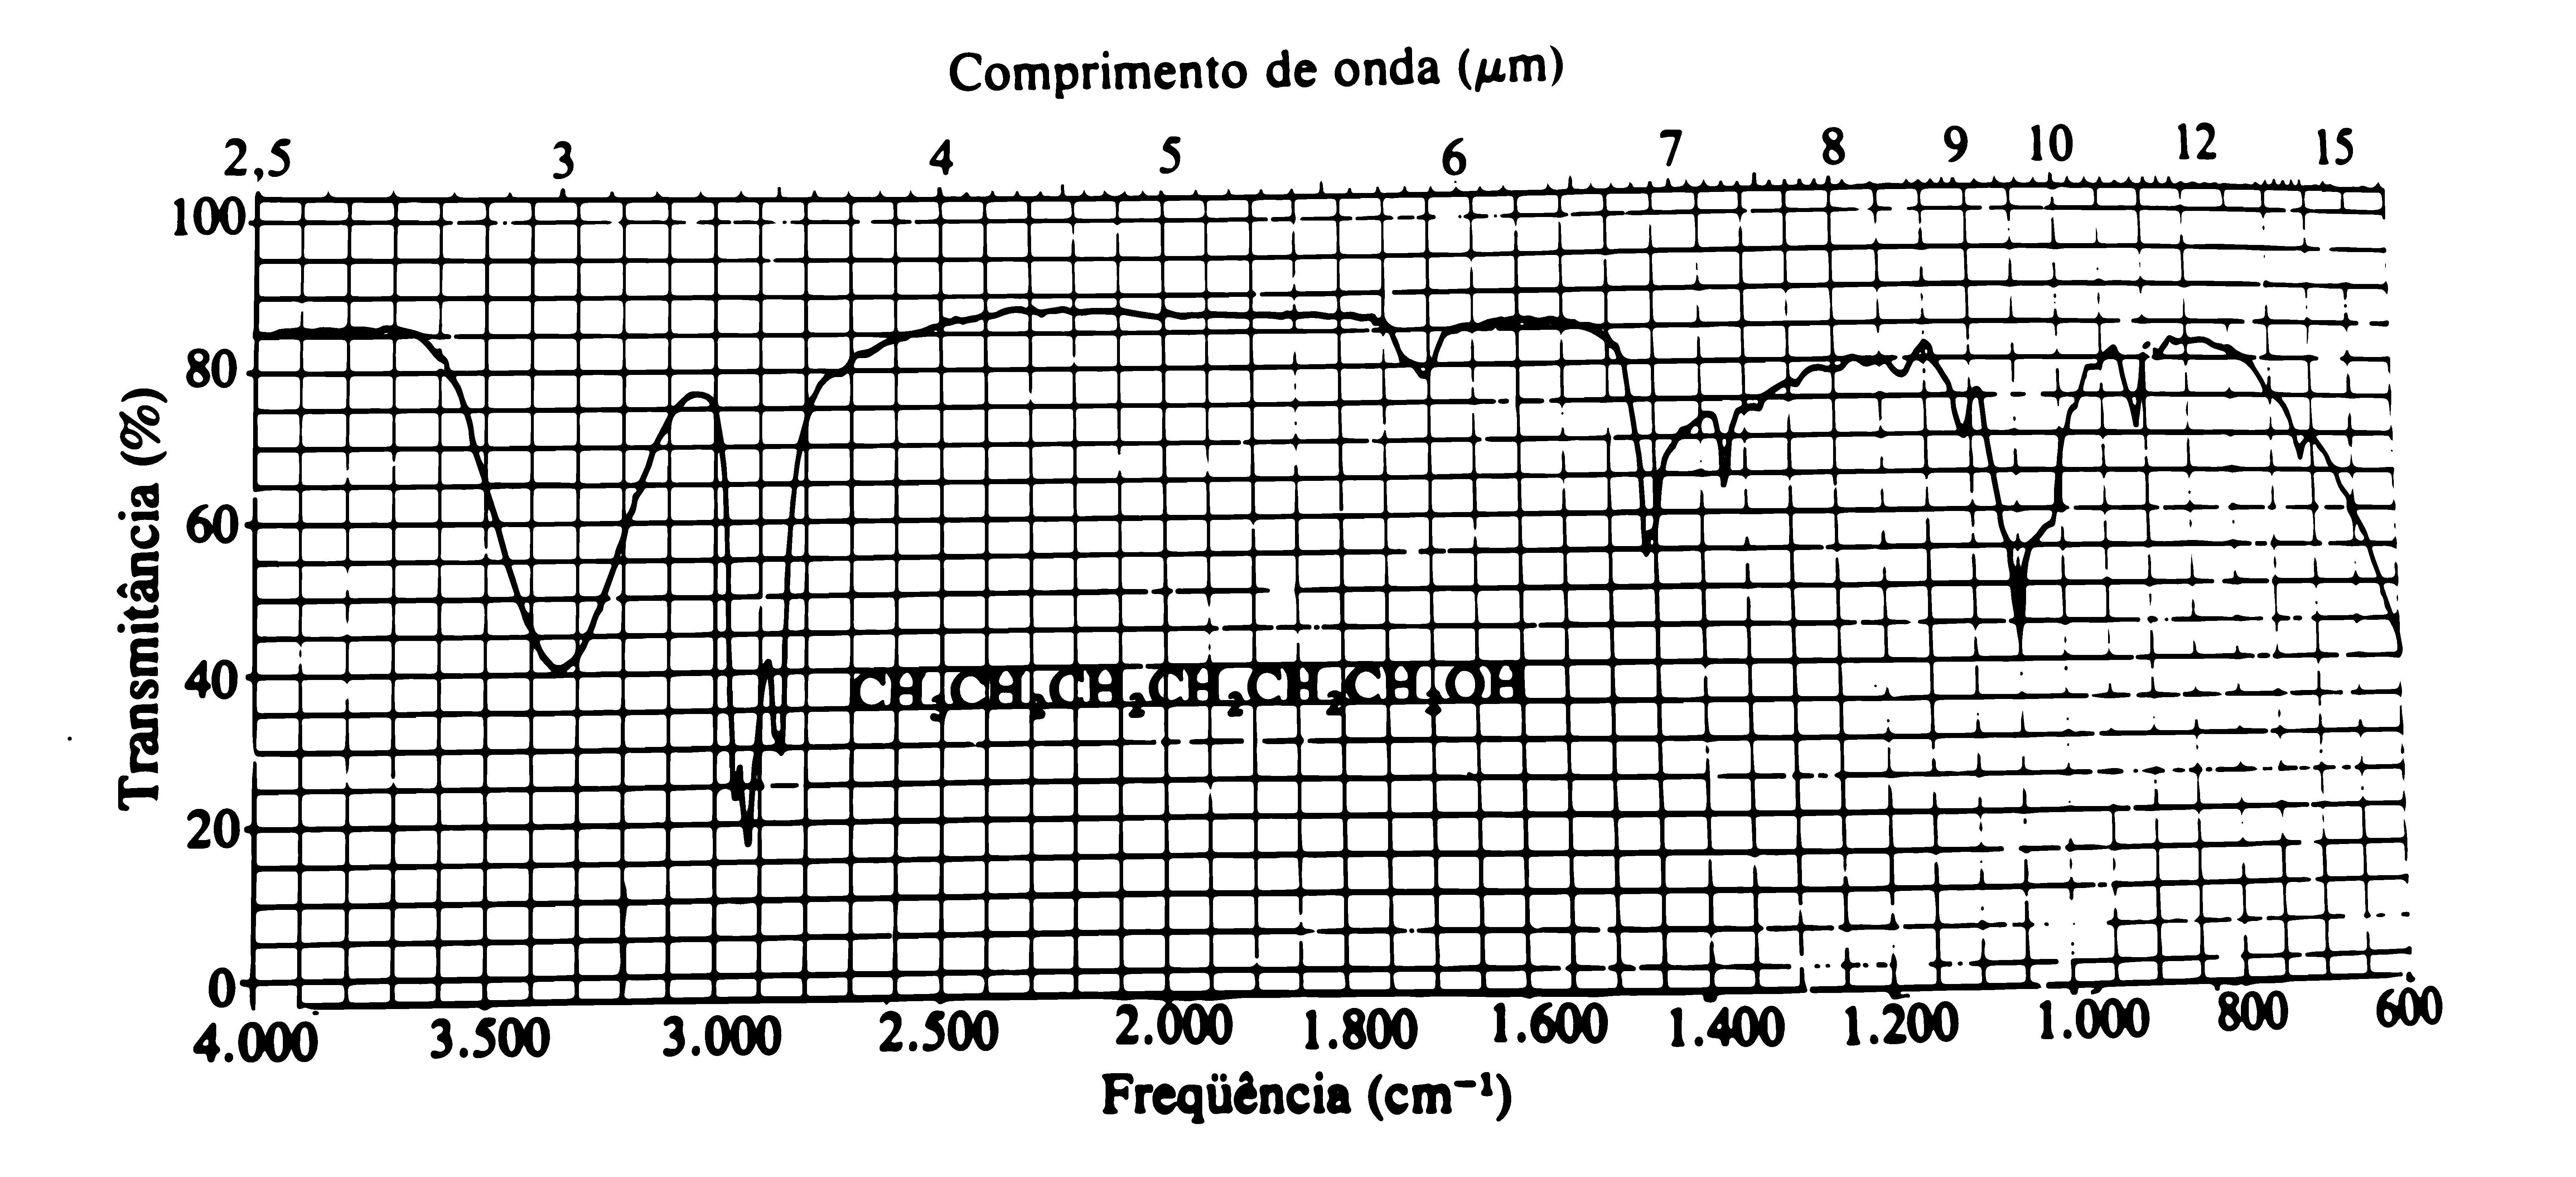
\includegraphics[width=0.9\textwidth,angle=0]{content/images/Figura_9_5.pdf}
    \caption{Espectro do 1-hexanol no infravermelho (filme líquido).}
    \label{figura_9_5}
\end{figure}

\begin{figure}[H]
    \centering
    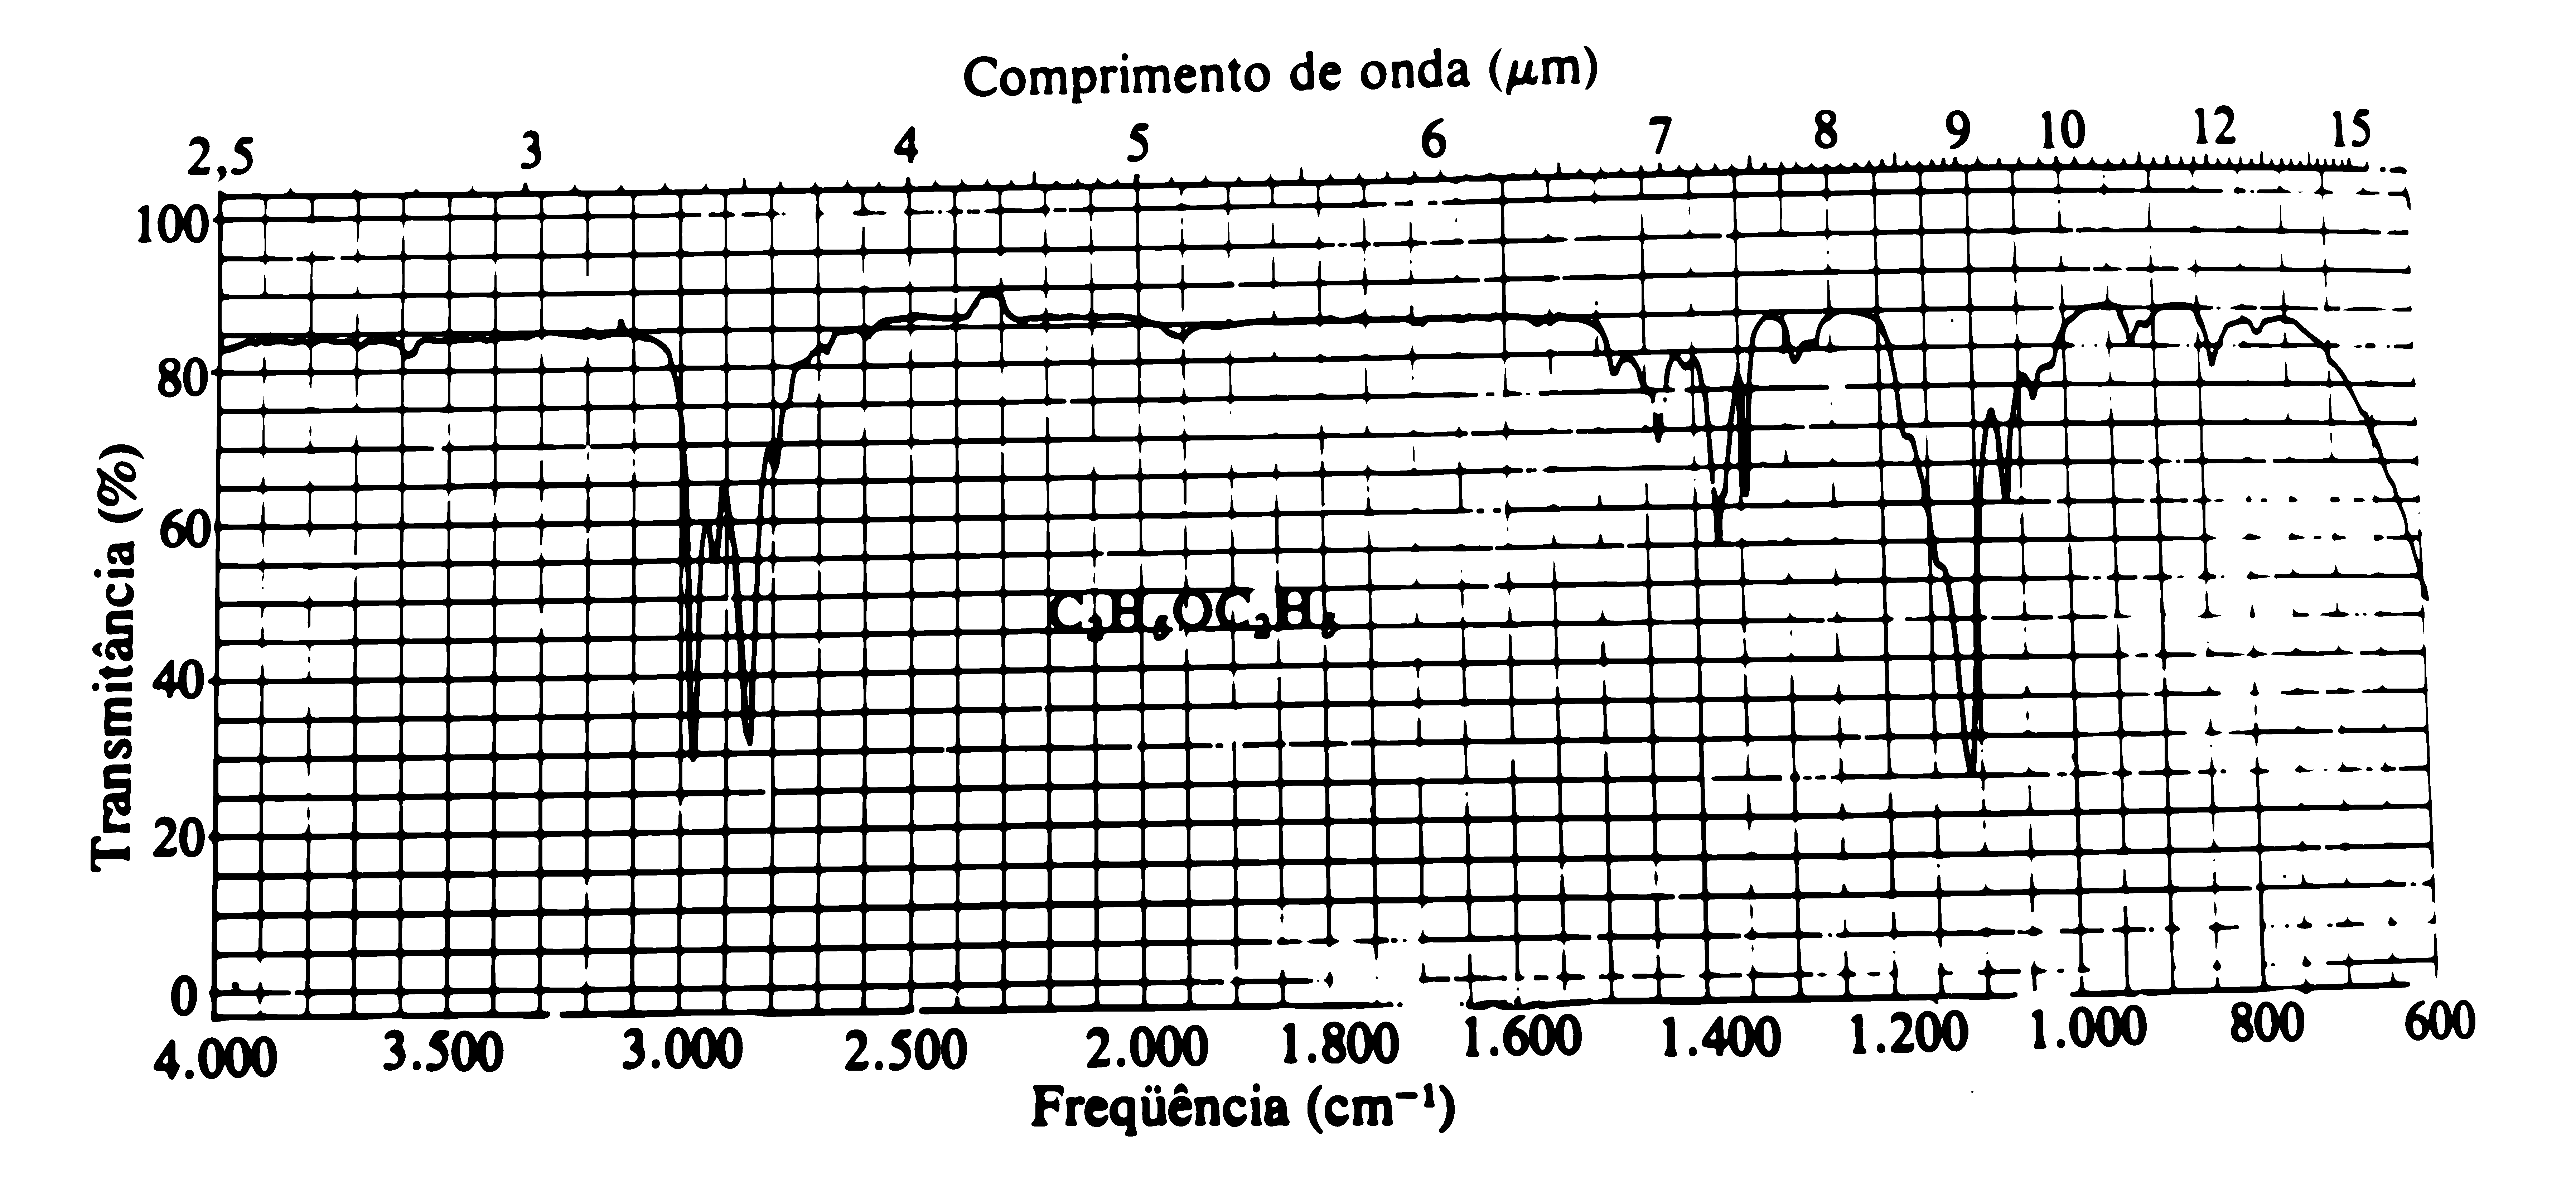
\includegraphics[width=0.9\textwidth,angle=0]{content/images/Figura_9_6.pdf}
    \caption{Espectro do dietil-éter no infravermelho (filme líquido).}
    \label{figura_9_6}
\end{figure}

\begin{figure}[H]
    \centering
    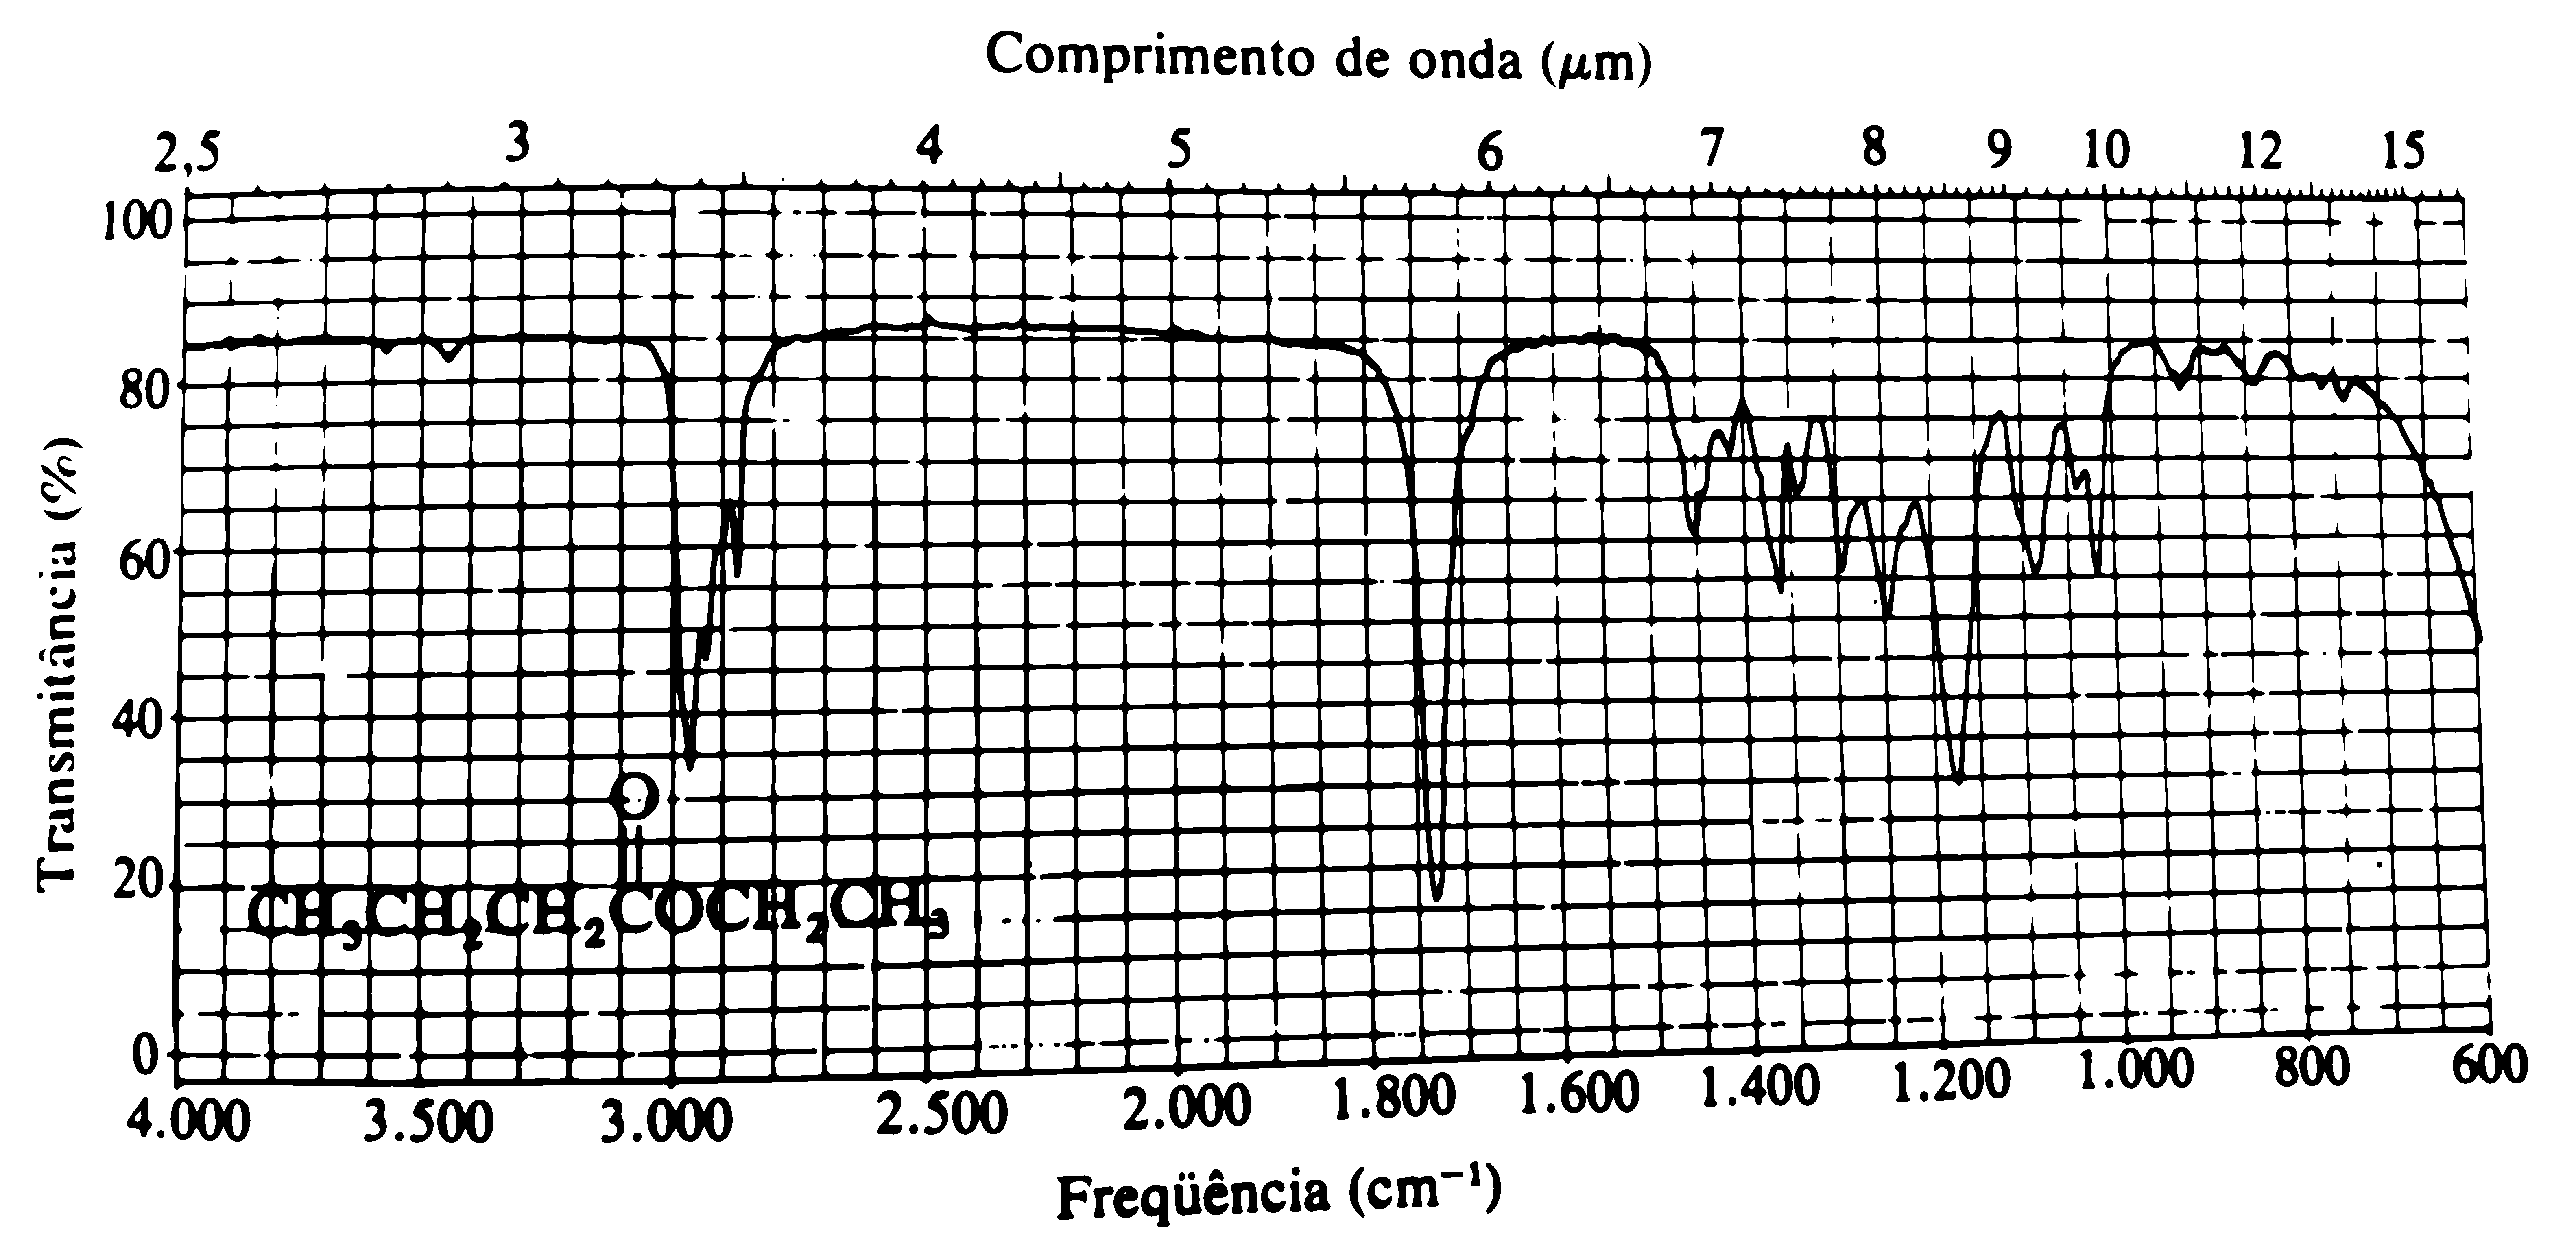
\includegraphics[width=0.9\textwidth,angle=0]{content/images/Figura_9_7.pdf}
    \caption{Espectro do butirato no infravermelho (filme líquido).}
    \label{figura_9_7}
\end{figure}

Nos espectros de RMN a intensidade do pico é proporcional ao número de prótons que contribuem para aquele pico. Nos espectros no infravermelho não existe uma relação deste tipo. A intensidade de um dado pico no infravermelho é proporcional à variação do momento de dipolo da molécula causada pela absorção. Esta variação não é previsível, em geral, em uma forma simples, entretanto algumas generalizações feitas podem ser úteis.

Primeiro, a vibração de uma ligação polar (\ch{C-O}, \ch{C=O}, \ch{C-Br}) deve levar a uma variação maior do momento de dipolo da molécula do que a de uma ligação menos polar (\ch{C-C}, \ch{C-N}, \ch{C=N}) e, portanto, os grupos mais polares levam, geralmente, a bandas de absorção mais fortes. Segundo, a vibração através de um centro de simetria não causa mudança no momento de dipolo e tais vibrações levam a absorções muito fracas (ou a nenhuma absorção) no infravermelho. Assim, a absorção de deformação axial a cerca de 1.650 cm$^{-1}$ é muito fraca no etileno e no tetrametil-etileno mas é mais forte no propano e no isobutileno.

Em geral os sistemas conjugados absorvem a frequência mais baixas do que os sistemas não conjugados. Por exemplo, os alquenos absorvem a 1670-1640 cm$^{-1}$ enquanto que os alquenos conjugados com um grupo carbonila ou outra ligação dupla absorvem a cerca de 1.600 cm$^{-1}$. Estas variações podem ser interpretadas em termos de formas ressonantes, como no butadieno:

\begin{figure}[H]
    \centering
    \schemestart
        \chemfig[][scale=0.7]{CH_2=CH-CH=CH_2}
        \arrow{<->}
        \chemfig[][scale=0.7]{^{-}CH_2-CH=CH=CH_2^{+}}
    \schemestop
\end{figure}

\noindent contribuições das formas iônicas tendem a enfraquecer as ligações duplas e tornar mais fortes as ligações simples. Estas formas de ressonância contribuem relativamente pouco e as variações na frequências de absorção não são muito grandes.

Na prática a absorção do grupo carbonila no infravermelho é de grande importância. A absorção é forte (Por quê?) e ocorre em uma região onde usualmente não aparecem outras bandas. É, portanto, fácil de localizar e identificar. A frequência exata da absorção de \ch{C=O} depende de um certo número de variáveis bem conhecidas. Se a frequência puder ser determinada, poderemos inferir muito da estrutura do composto. Um éster absorve a frequência maior do que uma cetona que, por sua vez, absorve a maior frequência do que uma amida. Se uma cetona está em um anel a frequência de absorção é uma função do tamanho do anel. A frequência varia inversamente com o ângulo \ch{C-C-C} do grupamento carbonila. Em regra, as carbonilas em anéis de seis membros têm frequências de absorção de valor aproximadamente o mesmo que os compostos de cadeia aberta correspondentes, enquanto que a \textit{diminuição do tamanho do anel aumenta a frequência de 30 cm$^{-1}$ por cada átomo de carbono}. Esta tendência é ilustrada abaixo:

\begin{figure}[H]
    \centering
    \chemnameinit{}
    \chemname{\chemfig[][scale=0.7]{R-C(=[2]O)-R}}{\footnotesize{1715 cm$^{-1}$}}
    \qquad
    \chemnameinit{}
    \chemname{\chemfig[][scale=0.7]{*6(----(=[2]O)--)}}{\footnotesize{1715 cm$^{-1}$}}
    \qquad
    \chemnameinit{}
    \chemname{\chemfig[][scale=0.7]{*5(---(=O)--)}}{\footnotesize{1745 cm$^{-1}$}}
    \qquad
    \chemnameinit{}
    \chemname{\chemfig[][scale=0.7]{*4(--(=[1]O)--)}}{\footnotesize{1775 cm$^{-1}$}}
\end{figure}

Quando uma ligação dupla carbono-carbono está em conjugação com uma carbonila esta \textit{conjugação abaixa de 30 cm$^{-1}$ a frequência observada da carbonila}. Este efeito é ilustrado nos exemplos seguintes.

\begin{figure}[H]
    \centering
    \chemnameinit{}
    \chemname{\chemfig[][scale=0.7]{CH_3(-[7]CH(-[5]CH_3)-CH_2-C(=[2]O)(-CH_3))}}{\footnotesize{1715 cm$^{-1}$}}
    \qquad
    \chemnameinit{}
    \chemname{\chemfig[][scale=0.7]{CH_3(-[7]C(-[5]CH_3)=CH-C(=[2]O)(-CH_3))}}{\footnotesize{1685 cm$^{-1}$}}
    \qquad
    \chemnameinit{}
    \chemname{\chemfig[][scale=0.7]{*6(---O-(=[2]O)--)}}{\footnotesize{1735 cm$^{-1}$}}
    \qquad
    \chemnameinit{}
    \chemname{\chemfig[][scale=0.7]{*6(---O-(=[2]O)-=)}}{\footnotesize{1705 cm$^{-1}$}}
\end{figure}

Vemos, então, que a frequência da carbonila no espectro no infravermelho de um composto de estrutura desconhecida pode fornecer informações úteis. Podemos saber o grupo funcional do qual a carbonila faz parte, se o grupo carbonila faz parte de uma anel ou se é conjugado.

Embora muitas bandas não possam ser relacionadas a uma vibração específica, o estudo comparativo de aproximadamente 125.000 espectros de compostos de estrutura conhecida resultou em muitas correlações empíricas que podem ser utilizadas para reconhecer-se características estruturais de compostos desconhecidos pelo exame de seus espectros no infravermelho. Na Tabela \ref{tabela_9_3} são fornecidas algumas frequências características de absorção de grupos funcionais no infravermelho. (Um quadro mais completo é dado no Apêndice).

\noindent \textbf{Comparações espectrais}

\noindent Os espectros de compostos no infravermelho contêm bandas de formas e tamanhos variados. Isto permite que um espectro no infravermelho possa ser usado como 'impressão digital' de um composto. Em caso de compostos de complexidade moderada, a \textit{superposição dos espectros de um composto desconhecido e de um composto conhecido estabelece a identidade entre os dois}. Esta comparação não é prove suficiente em dois casos especiais. Primeiro, moléculas diferentes de estrutura simples muito semelhantes, tais como pentadecano e hexadecano podem ter diferenças insignificantes e difíceis de detectar em seus espectros. Segundo, em moléculas muito grandes e complicadas, como polímeros e peptídeos, a resolução obtida no espectro é usualmente insuficiente para permitir uma identificação positiva.

\begin{table}[H]
\centering
\caption{Frequências de absorção características de grupos funcionais no infravermelho.}
\label{tabela_9_3}
    \begin{tabular*}{\textwidth}{cccc}
        \toprule
        Grupo & Classe do compostos & Frequência (cm$^{-1}$) & Intensidade \\
        \midrule
        \ch{C-H} & Alcano & 2965-2850 (deformação axial) & Forte \\
         & \ch{-CH3} & 1450 (deformação angular & Média \\
         &  & 1380 (deformação angular) & Média \\
         & \ch{-CH2-} & 1465 & Média \\
         & Alqueno & 3095-3010 (deformação axial) & Média \\
         &  & 700-1000 (deformação angular) & Forte \\
         & Alquino & \sim 3300 & Forte \\
         & Aldeído & 2900-2820 & Fraca \\
         &  & 2775-2700 & Fraca \\
        \ch{C-C} & Alcano & 700-1200 (geralmente não é útil) & Fraca \\
         & Alqueno$^a$ & 1680-1620 & Variável \\
         & Alquino$^a$ & 2260-2100 & Variável \\
        \ch{C=O}$^a$ & Cetona & 1715 & Forte \\
         & Aldeído & 1725 & Forte \\
         & Ácido carboxílico & 1710 & Forte \\
         & Ester & 1735 & Forte \\
         & Amida & 1650 & Forte \\
         & Anidrido & 1820 e 1760 & Forte \\
        \ch{C-O} & Álcool, éster, ácido carboxílico, éter & 1300-1000 & Forte \\
        \ch{O-H} & \underline{Álcool} &  &  \\
         & Monômero & 3650-3590 & Variável e aguda \\
         & Em ligação hidrogênio & 3400-3200 & Forte e larga \\
         & \underline{Ácido carboxílico} &  & \\
         & Em ligação hidrogênio & 3300-3500 & Variável e larga \\
        \ch{N-H} & Amina e amida primárias & \sim 3500 (deformação axial)$^b$ & Média \\
         & Amine e amida secundárias & 3500 (deformação axial)$^b$ & Média \\
        \ch{C+N} & Nitrila$^a$ & 2260-2240 & Média \\
        \ch{C-X} & Fluoreto & 1400-1000 & Forte \\
         & Cloreto & 800-600 & Forte \\
         & Brometo & 600-500 & Forte \\
         & Iodeto & \sim 500 & Forte \\
        \bottomrule
        \multicolumn{4}{p{0.98\textwidth}}{$^a$Não conjugada. Conjugação com ligações múltiplas abaixam de 30 cm$^{-1}$ a frequência de deformação axial.}\\
       \multicolumn{4}{p{0.98\textwidth}}{$^b$Mais baixa se em ligação hidrogênio.}
    \end{tabular*}
\end{table}

\section{INTERPRETAÇÃO DOS ESPECTROS}
Embora, não existam regras rígidas para a interpretação de um espectro no infravermelho, algumas diretrizes poder ser úteis.

\begin{enumerate}
    \item \textit{Comece pelo lado esquerdo do espectro e faça um exame preliminar da região 4000-1500 cm$^{-1}$}. Não tente interpretar com detalhes a ragião de deformação axial da ligação \ch{C-H} próxima a 3000 cm$^{-1}$. Assinale, tentativamente, todas as demais bandas. As vibrações de deformação axial características de grupos funcionais muito importantes, como \ch{OH}, \ch{NH}, \ch{C=O} e \ch{C=C}, ocorrem nesta região. Lembre-se que a ausência de absorções nas regiões habituais de vibração é muito importante para reduzir o número de compostos que deveremos considerar a seguir.
    \item \textit{Sempre que possível, o assinalamento de bandas feito acima deve ser confirmado pelo exame de outras porções do espectro.}
    \item \textit{Examine a região de deformação axial do \ch{CH} logo acima de 3000 cm$^{-1}$ para determinar se o hidrogênio está ligado a carbono insaturado.} Se tal indicação é encontrada, tente descobrir o tipo de insaturação em outras regiões do espectro.
    \item \textit{Examine o espectro na região 1500-600 cm$^{-1}$ para um a indicação de outros grupos funcionais, tais como éteres ou halogênios.} Este é um passo importante se o item 1 não revelou a presença dos grupos funcionais mais óbvios.
\end{enumerate}

\begin{figure}[H]
    \centering
    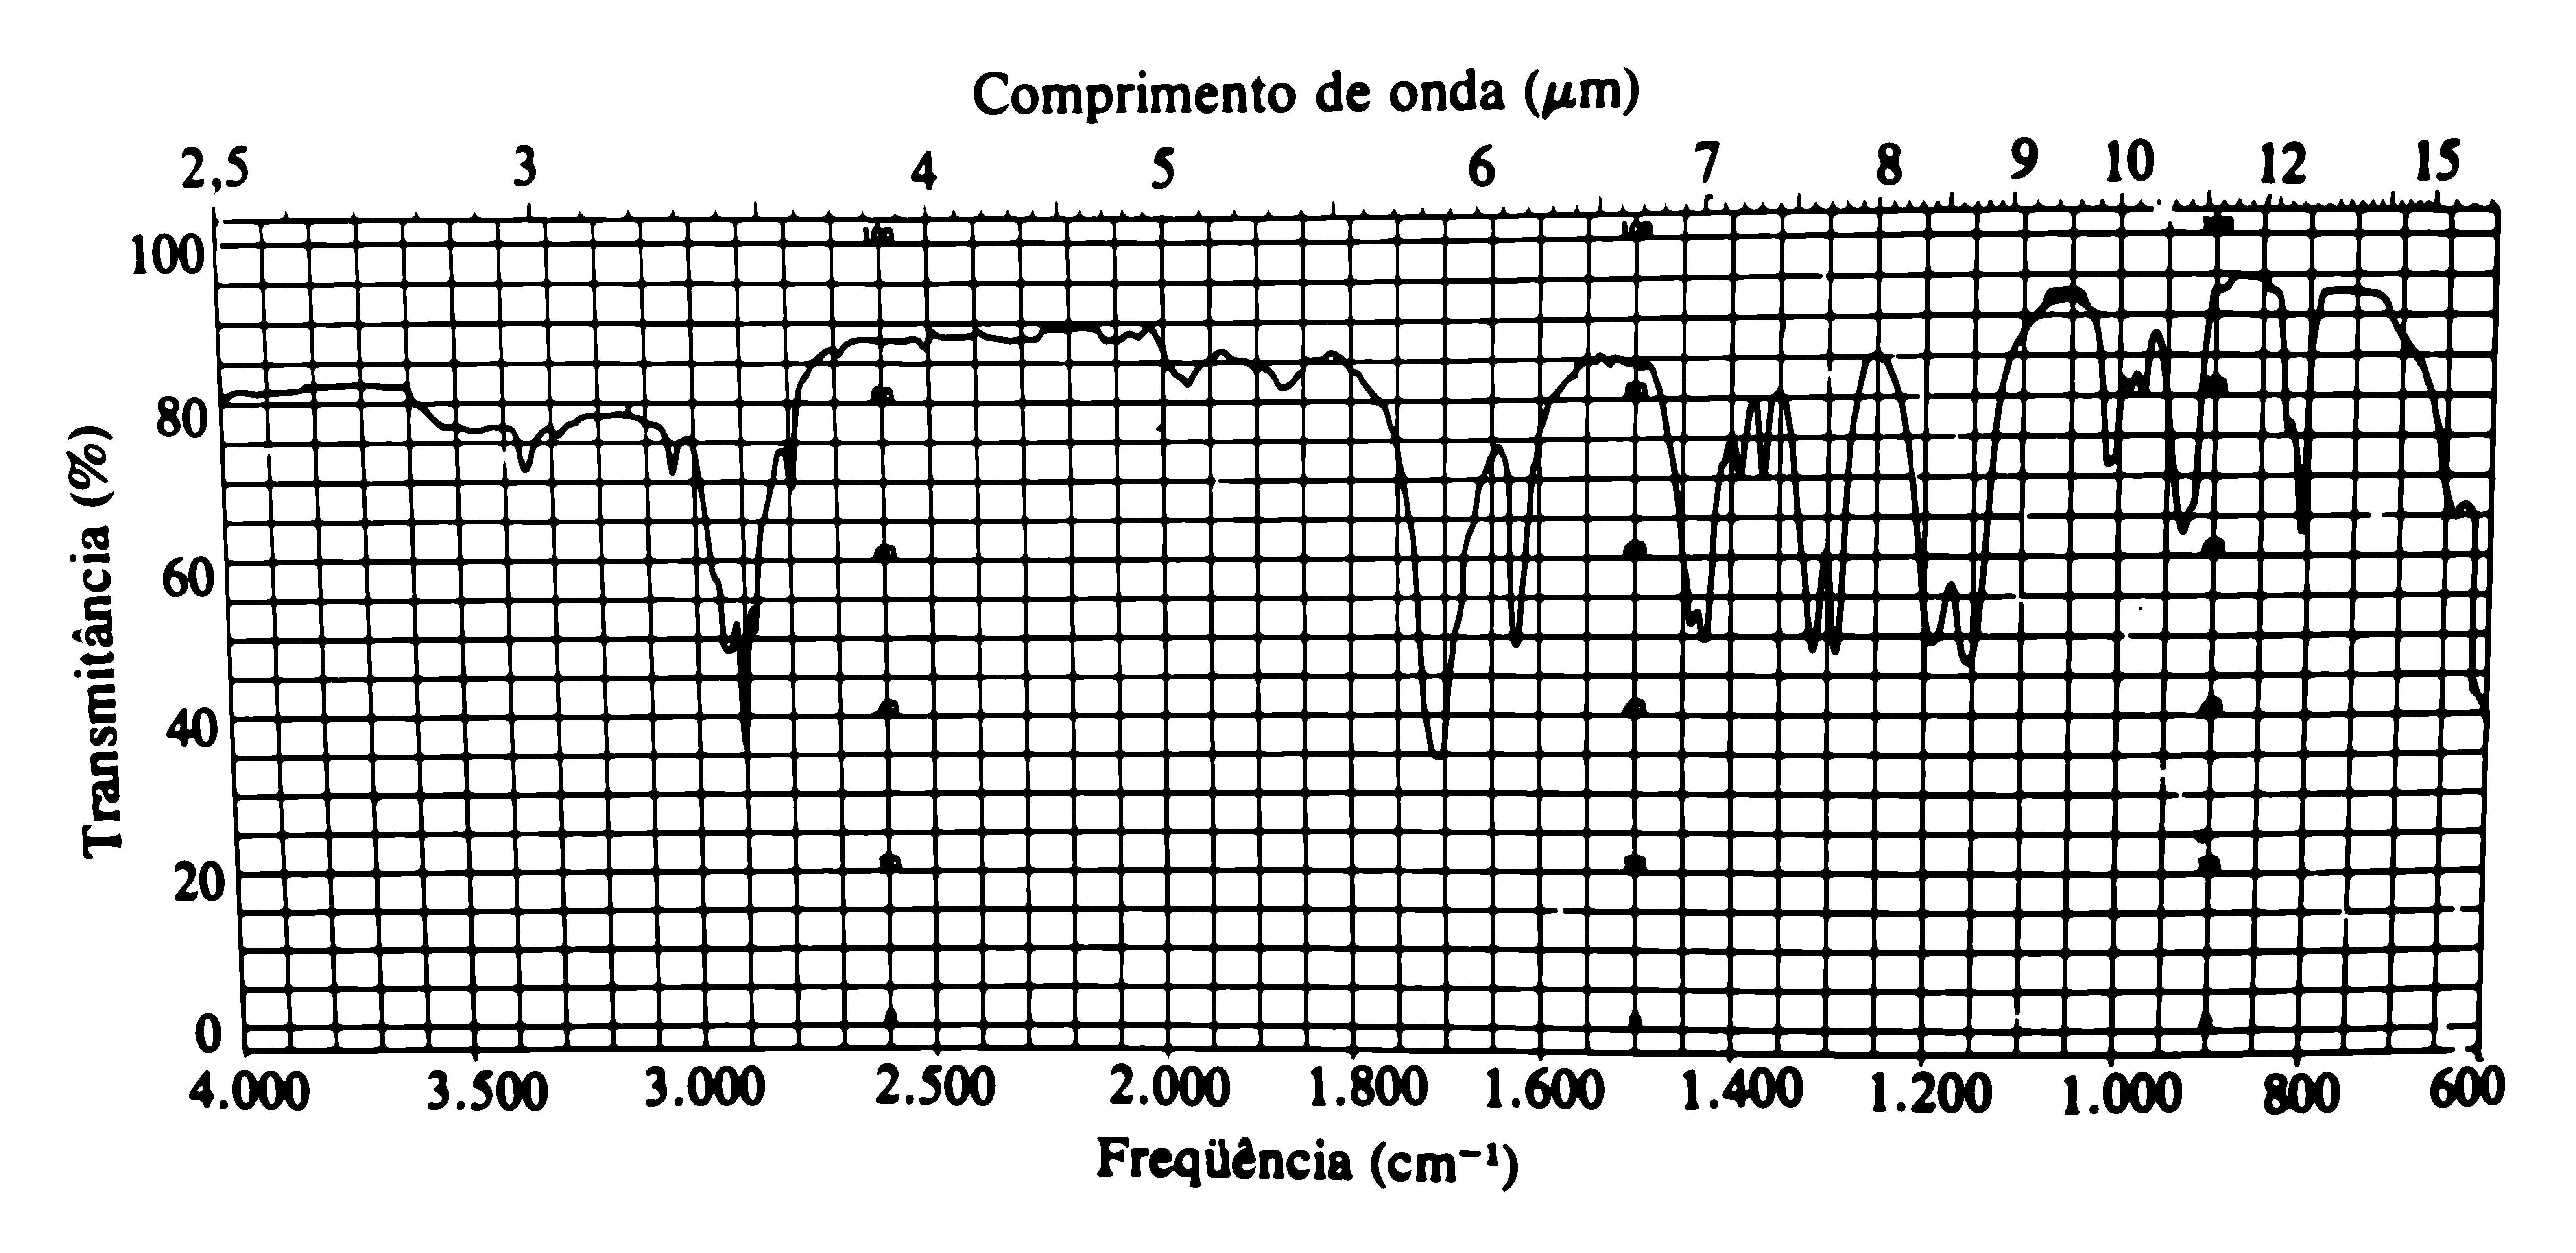
\includegraphics[width=0.9\textwidth,angle=0]{content/images/Figura_9_8.pdf}
    \caption{Espectro no infravermelho de um composto desconhecido (filme líquido).}
    \label{figura_9_8}
\end{figure}

Como um exemplo da aplicação dessa diretrizes consideremos o exemplo do espectro no infravermelho de um composto desconhecido apresentado na Figura \ref{figura_9_8}. Aplicação do item 1 revela uma banda de \ch{C=O} a 1708 cm$^{-1}$ a de \ch{C=C} a 1625 cm$^{-1}$. A banda de \ch{C=O} a 1708 cm$^{-1}$ é consistente  com a estrutura de um aldeído, cetona, ácido carboxílico ou éster. O exame de outras partes do espectro (item 2) nos permitirá a descoberta do tipo da carbonila. Um aldeído pode ser confirmado peloa presença de uma banda, ou melhor, um par de bandas a 2800 e 2700 cm$^{-1}$ (veja a Figura \ref{figura_9_9}). Um ácido carboxílico mostra uma banda muito larga característica de \ch{OH} a 3500-2500 cm$^{-1}$ (veja a Figura \ref{figura_9_11}) e foi eliminado pelo exame preliminar desta região que indicou a ausência de absorção de \ch{OH}. Um éter sempre exibe uma ou duas bandas fortes na região 1300-100 cm$^{-1}$ (veja a Figura \ref{figura_9_7}). Observe na Figura \ref{figura_9_8} as duas bandas fortes próximas a 1200 cm$^{-1}$, sugerindo fortemente que nosso desconhecido é um éster. A posição da carbonila do éster a 1708 cm$^{-1}$ sugere que o \ch{C=O} é conjugado. Olhando o espectro novamente (item 3) encontramos evidencia adicional na região do \ch{CH} olefínico acima de 3000 cm$^{-1}$, na banda \ch{C=C} a 1625 cm$^{-1}$ e, provavelmente, também na região de deformação angular do \ch{CH} olefínico a 930 cm$^{-1}$. Neste ponto é razoável afirmar que nosso exemplo desconhecido é um éster $\alpha$,$\beta$-insaturado.

Como um segundo exemplo, reexaminemos o espectro do dietil-éter, mostrado na Figura \ref{figura_9_6}. Suponha que a identidade deste composto não tivesse sido revelada. O exame do espectro na região 4000-1500 cm$^{-1}$ revela apenas a existência de deformações axiais de \ch{CH}. Aplicando o item 3, notamos a ausência de \ch{CH} olefínico acima de 3000 cm$^{-1}$. Aplicando o item 4, notamos a presença de uma banda forte próxima a 1100 cm$^{-1}$ que não existe no espectro do hidrocarbonetos simples (veja a Figura \ref{figura_9_2}). Esta banda está na região de \ch{C-O} (Tabela \ref{tabela_9_3} e Apêndice) e, na ausência de \ch{C=O} e \ch{O-H}, podemos concluir que o composto é um éter.

\section{EXEMPLOS DO USO DA ESPECTROSCOPIA NO INFRAVERMELHO}
Para ilustrar como a espectroscopia no infravermelho pode ser usada para ajudar a resolver problemas encontrados no laboratório examinemos duas situações tipicas.

\noindent \textit{Exemplo}: uma garrafa, contendo 100 g de butanal, foi comprada de um fornecedor. Este declarava que o material era 99,9\% puro. Como este nível de pureza era insatisfatório para o comprador, este purificou o butanal isolando 0,1 g de impurezas. Como um espectrofotômetro de infravermelho estava disponível, os espectros do butanal e da impureza no infravermelho foram obtidos.

O espectro do butanal puro no infravermelho está Figura \ref{figura_9_9}. A absorção da carbonila está a 1730 cm$^{-1}$, como deveríamos esperar para um aldeído alifático. Duas bandas devidas à deformação axial do \ch{C-H} do grupo aldeído são encontradas a 2800 e 2700 cm$^{-1}$.

O espectro da impureza no infravermelho aparece na Figura \ref{figura_9_10}. Absorção forte da carbonila é encontrada a 1710 cm$^{-1}$. Esta absorção (e o fato de que absorções que esperaríamos para outros grupos tais como \ch{-CHO} e \ch{-COOH} estão ausentes) sugerem que a impureza é uma cetona alifática saturada.

A impureza foi submetida à análise por RMN e o espectro obtido era idêntico ao da Figura 8.4. Assim, a impureza era butanona, um isômero do butanal.

\noindent\textit{Exemplo}: Deu-se aos estudantes de um laboratório de química orgânica uma amostra de manteiga rançosa e pediu-se que isolassem e identificassem o ingrediente que dá o odor rançoso característico. Eles acharam que a extração da manteiga rançosa com base removia o cheiro e a acidificação do extrato básico o regenerava. Após trabalho considerável, eles isolaram um composto ácido responsável pelo odor, cujo espectro no infravermelho é dado na Figura \ref{figura_9_11}. A absorção a 1770 cm$^{-1}$ é característica de um ácido carboxílico alifático. A vibração de deformação axial do \ch{OH} se estende de 3600 a 2500 cm$^{-1}$ por causa de ligação hidrogênio. Este tipo de banda de absorção, larga, é característico de um ácido carboxílico. Os estudantes descobriram que seu espectro era superponível ao espectro do ácido butírico. Outros dados químicos e espectroscópicos concordavam com este resultado.

\begin{figure}[h]
    \centering
    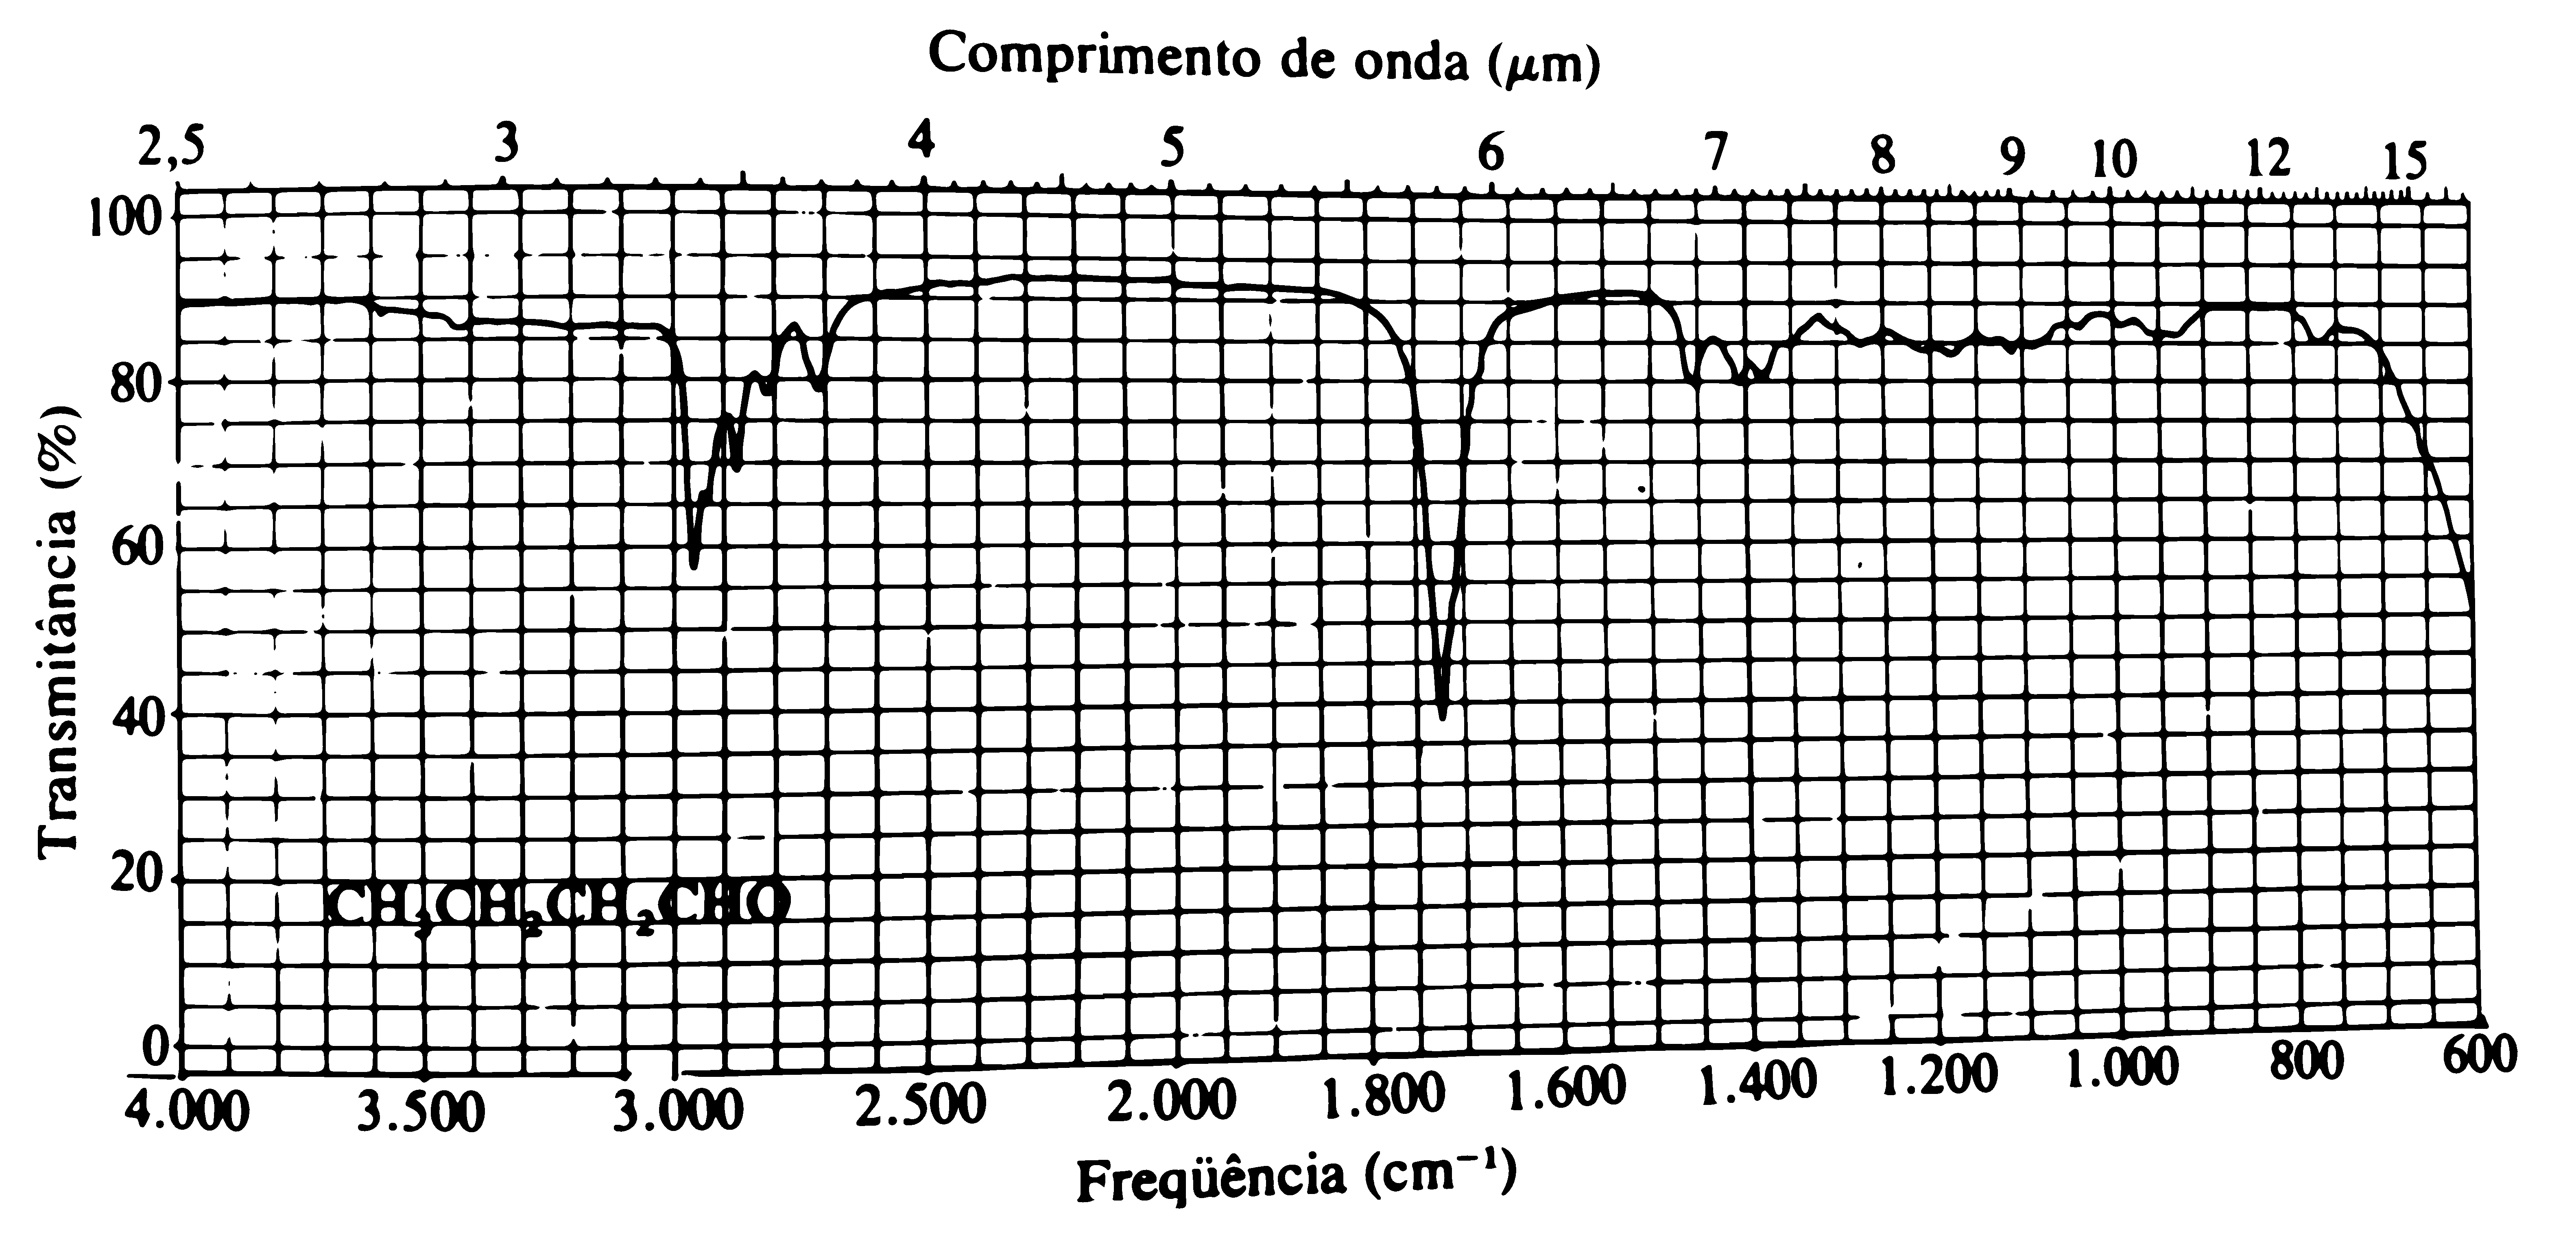
\includegraphics[width=0.9\textwidth,angle=0]{content/images/Figura_9_9.pdf}
    \caption{Espectro do butanal no infravermelho (filme líquido).}
    \label{figura_9_9}
\end{figure}

\begin{figure}[h]
    \centering
    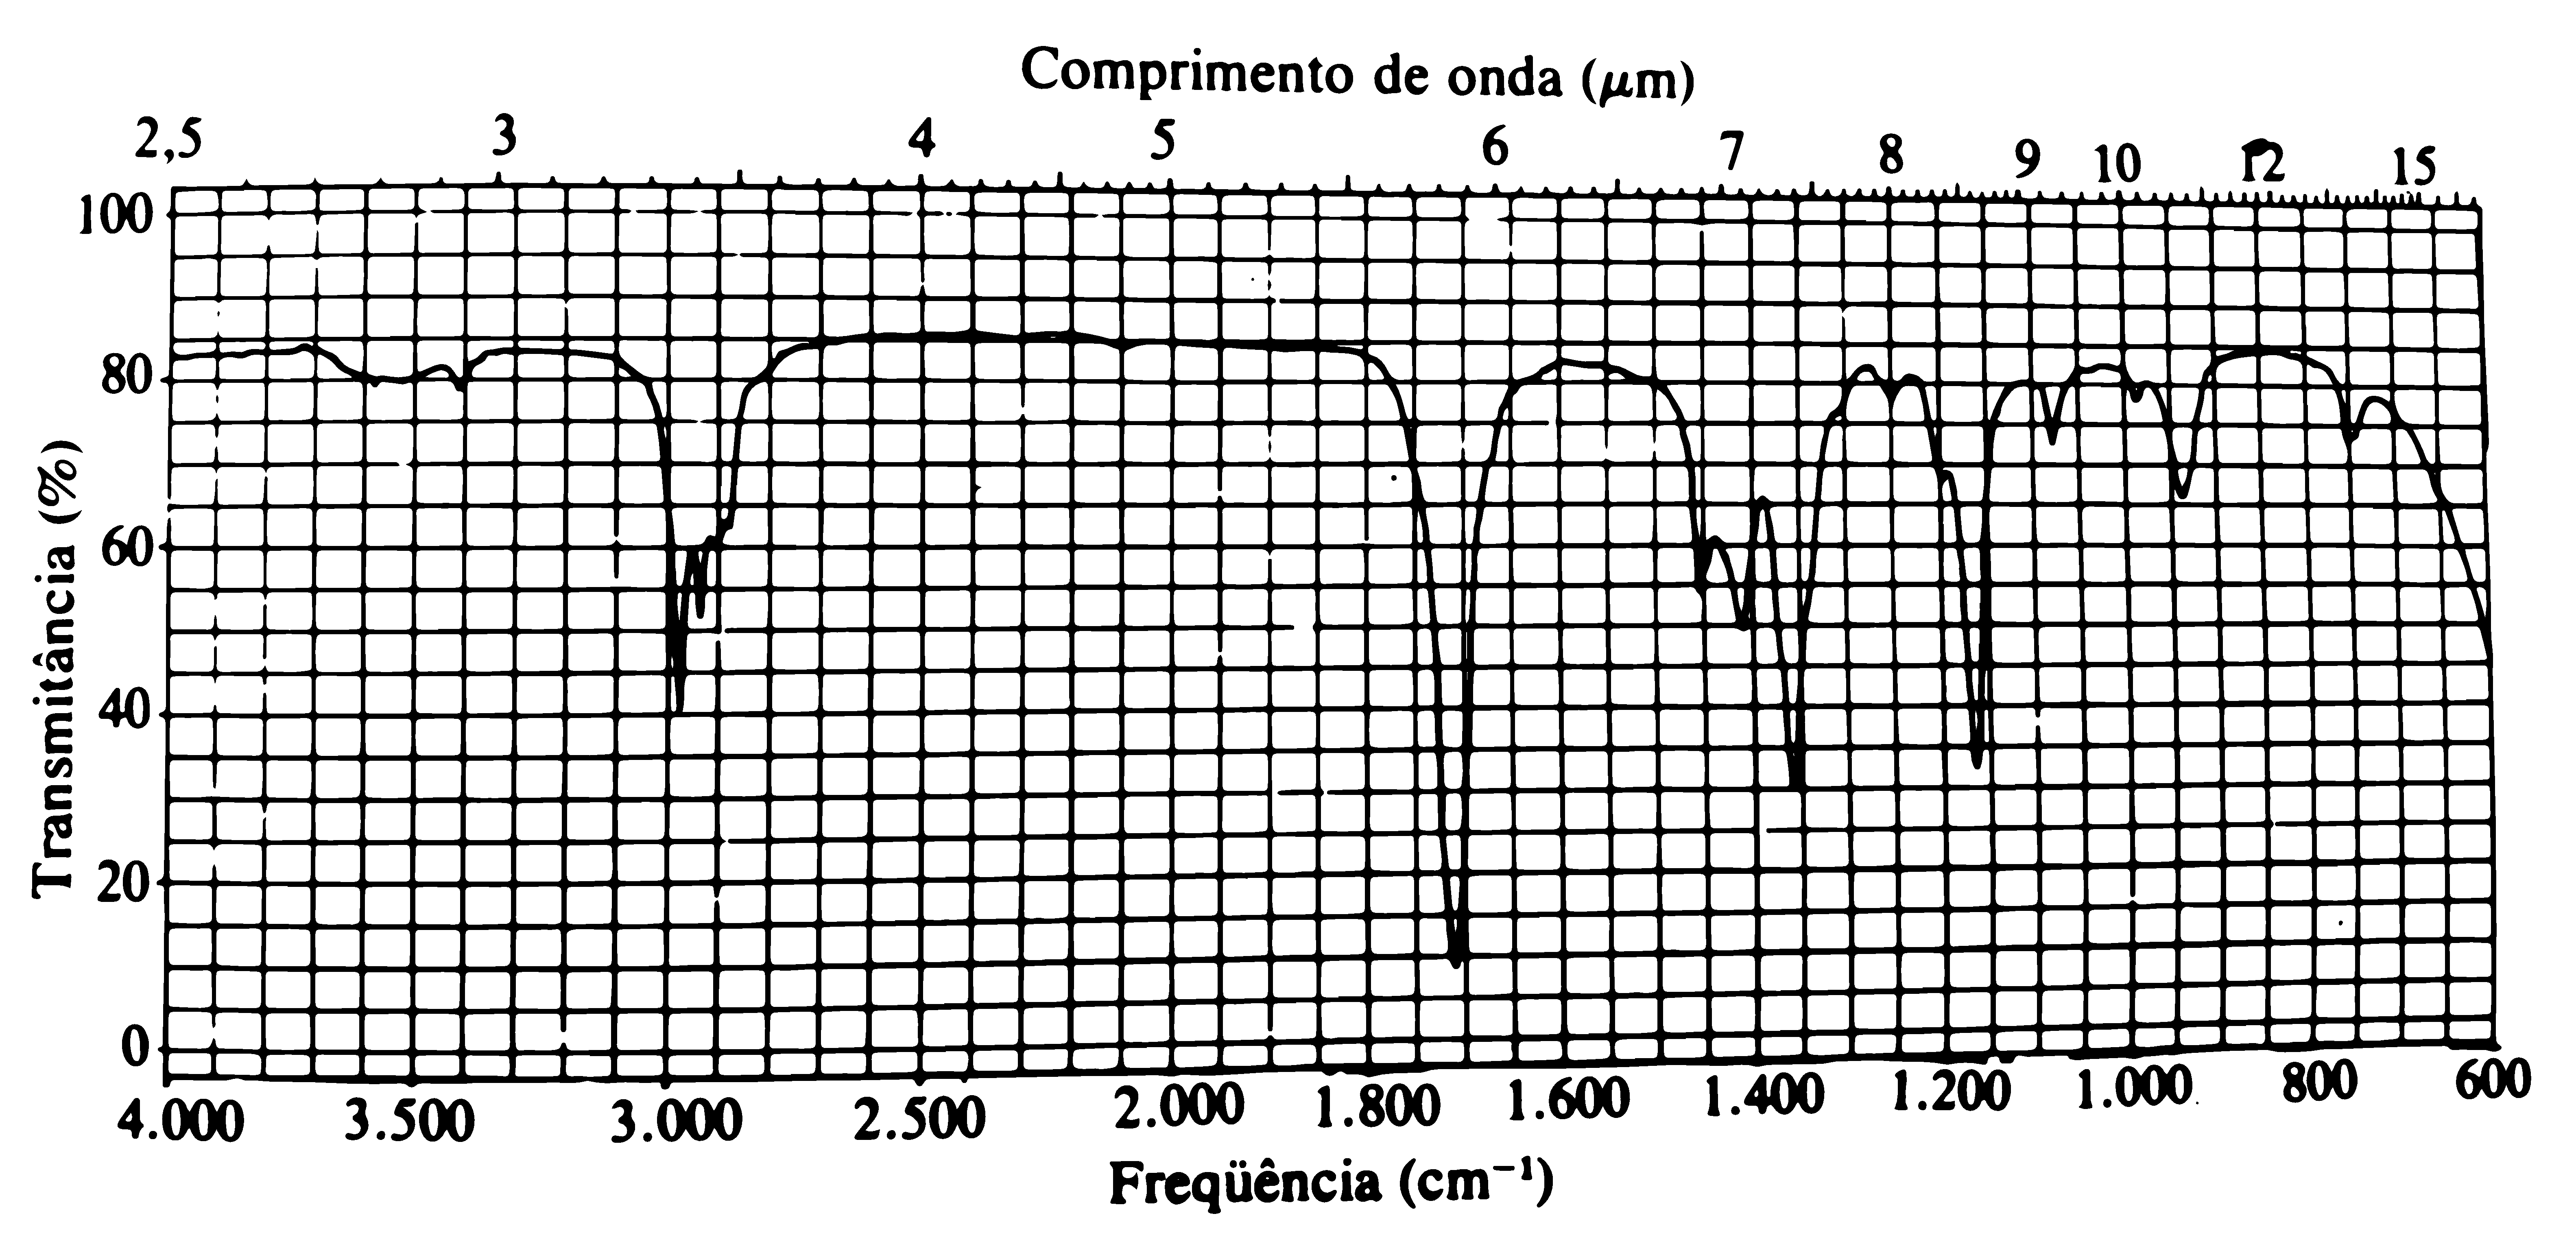
\includegraphics[width=0.9\textwidth,angle=0]{content/images/Figura_9_10.pdf}
    \caption{Espectro no infravermelho (filme líquido) de uma impureza isolada de butanal comercial e identificada como butanona.}
    \label{figura_9_10}
\end{figure}

\begin{figure}[h]
    \centering
    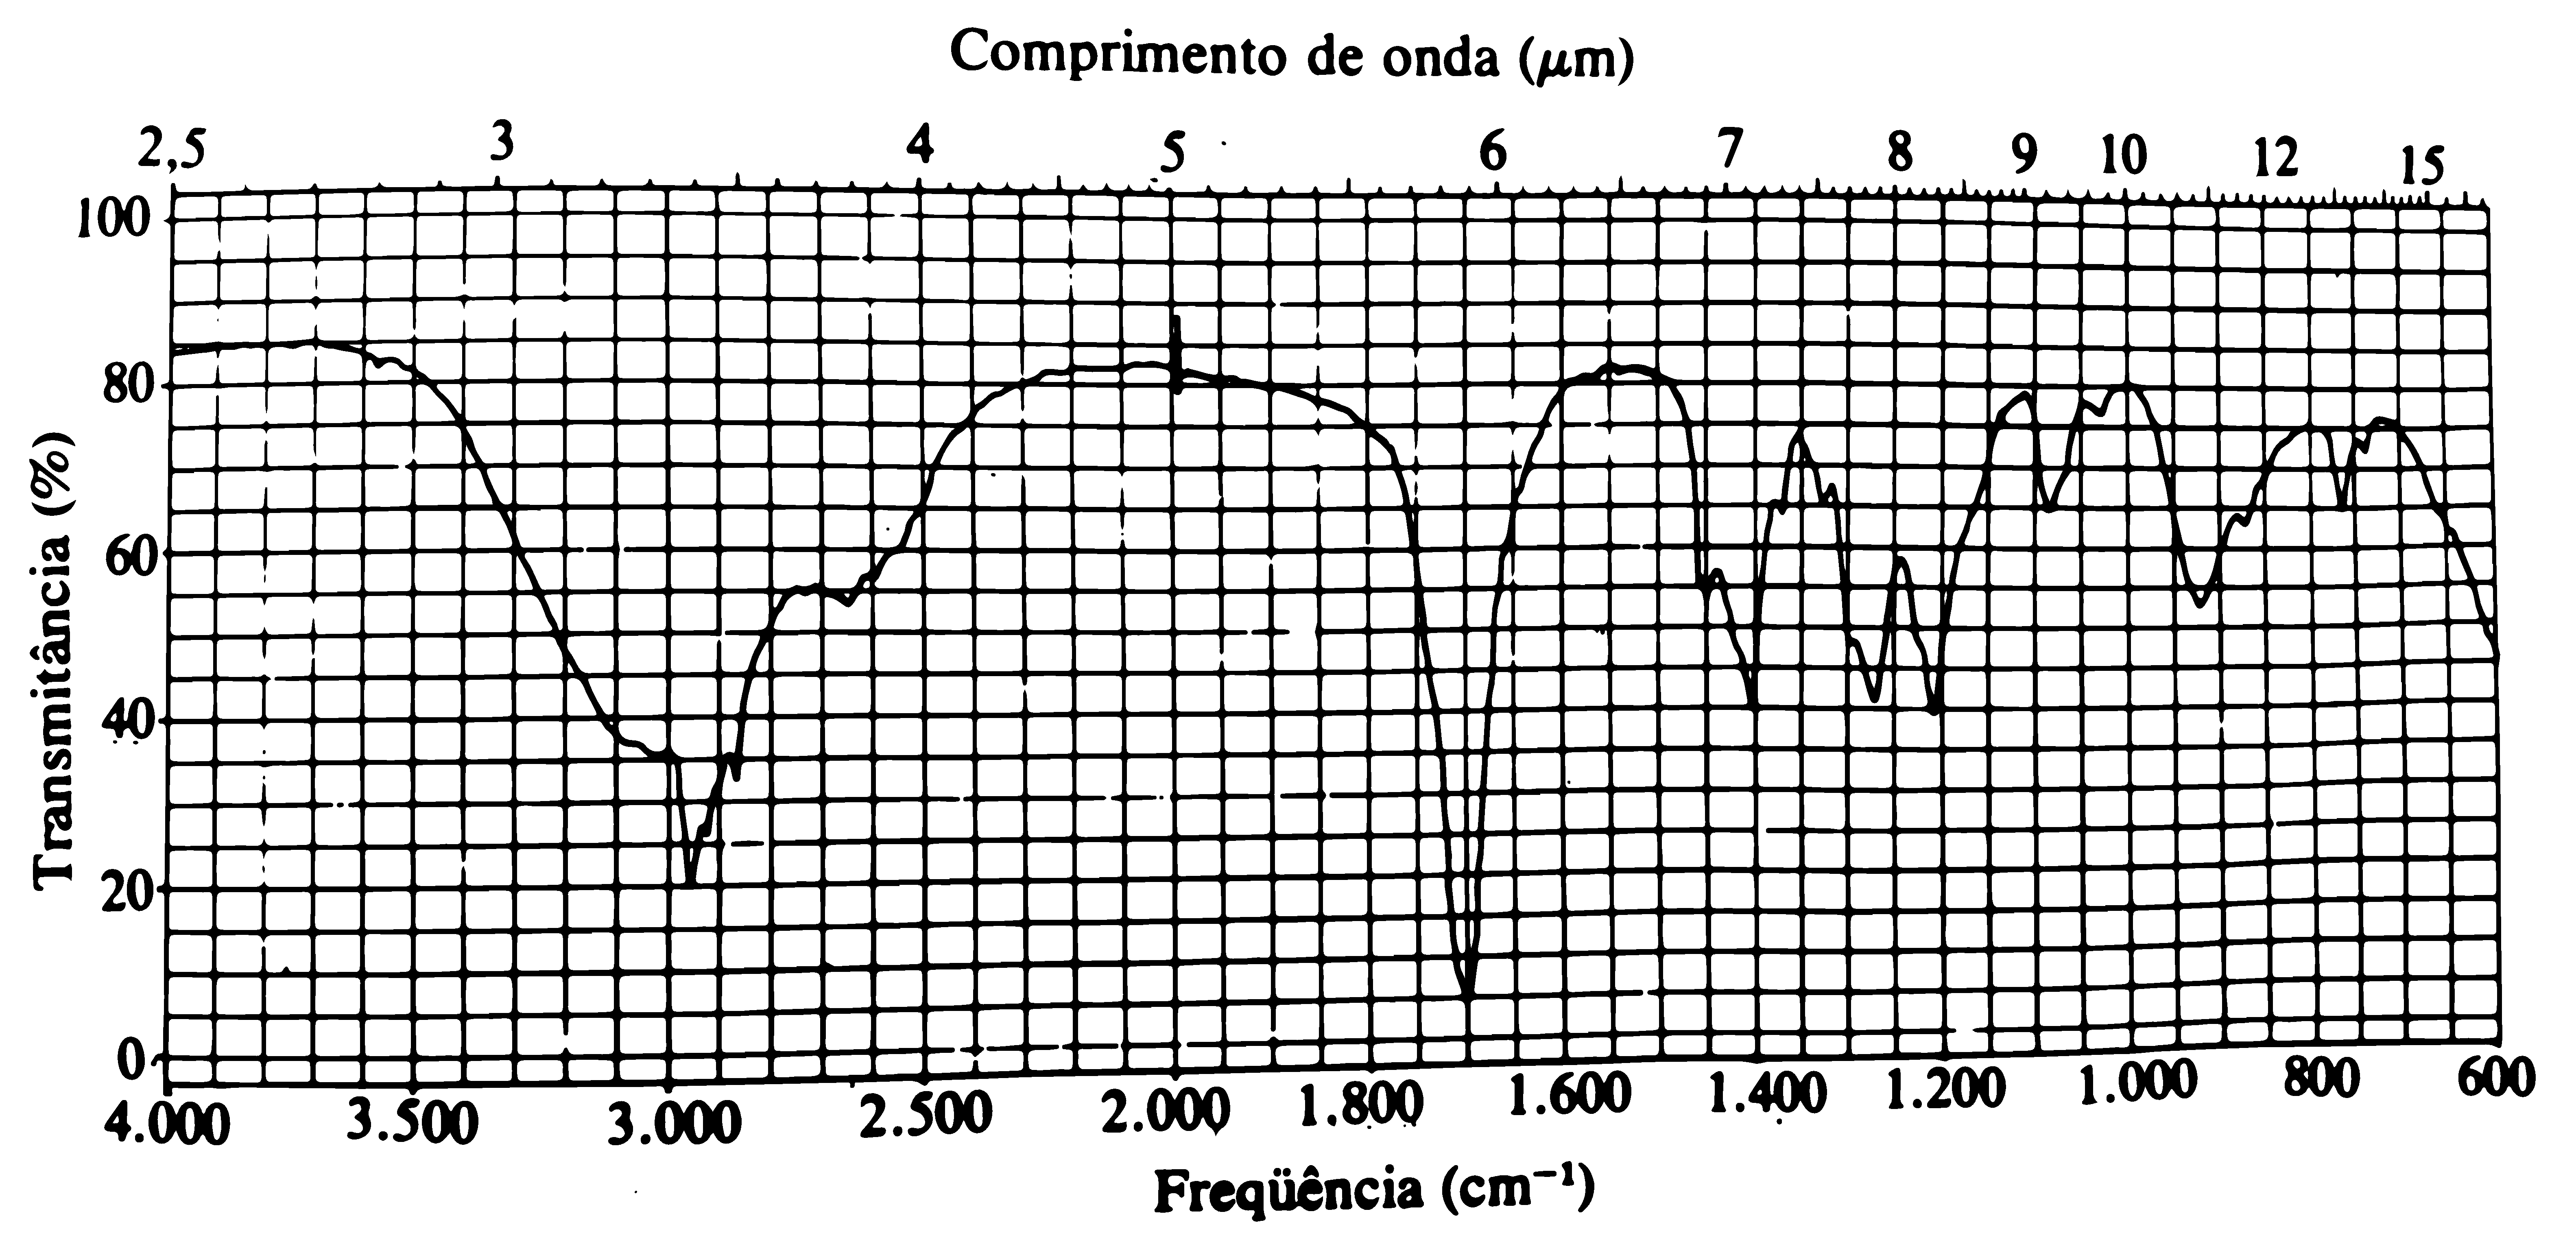
\includegraphics[width=0.9\textwidth,angle=0]{content/images/Figura_9_11.pdf}
    \caption{Espectro no infravermelho (filme líquido) de um composto desconhecido identificado como ácido butírico.}
    \label{figura_9_11}
\end{figure}

Existem outros classes de compostos, ainda não discutidos, para os quais pode-se obter informações e estruturais importantes a partir de seus espectros no infravermelho. Os fatos pertinentes serão apresentados quando estudarmos tais compostos. Veja o quadro no Apêndice para um sumário.
